%%=============================================================================
%% Methodologie
%%=============================================================================

\chapter{\IfLanguageName{dutch}{Methodologie}{Methodology}}%
\label{ch:methodologie}

%% TODO: In dit hoofstuk geef je een korte toelichting over hoe je te werk bent
%% gegaan. Verdeel je onderzoek in grote fasen, en licht in elke fase toe wat
%% de doelstelling was, welke deliverables daar uit gekomen zijn, en welke
%% onderzoeksmethoden je daarbij toegepast hebt. Verantwoord waarom je
%% op deze manier te werk gegaan bent.
%% 
%% Voorbeelden van zulke fasen zijn: literatuurstudie, opstellen van een
%% requirements-analyse, opstellen long-list (bij vergelijkende studie),
%% selectie van geschikte tools (bij vergelijkende studie, "short-list"),
%% opzetten testopstelling/PoC, uitvoeren testen en verzamelen
%% van resultaten, analyse van resultaten, ...
%%
%% !!!!! LET OP !!!!!
%%
%% Het is uitdrukkelijk NIET de bedoeling dat je het grootste deel van de corpus
%% van je bachelorproef in dit hoofstuk verwerkt! Dit hoofdstuk is eerder een
%% kort overzicht van je plan van aanpak.
%%
%% Maak voor elke fase (behalve het literatuuronderzoek) een NIEUW HOOFDSTUK aan
%% en geef het een gepaste titel.

\section*{Requirements analyse}
\label{sec:requirements-analyse}
Om de onderzoeksvraag te beantwoorden is het belangrijk 
de requirements te analyseren. De opgestelde requirements zullen de basis vormen voor de beoordeling, de vergelijkende analyse en de proof of concept.
 Deze vereisten zullen door diverse bronnen opgesteld worden. Als eerste
  zullen de belangrijkste vereisten in de voorgaande literatuurstudie onderzocht worden. Vervolgens zal er een vraag
   worden gesteld die mijn copromotor zal beantwoorden. De vraag bestaat uit: welke vereisten zijn volgens u belangrijk bij het kiezen van een 
   LCNC platform, en rangschik deze vereisten van belangrijk naar minder belangrijk. Op deze manier kan men een duidelijkbeeld weergeven van waarmee er rekening gehouden moet worden bij het evalueren van de Low-Code en/of No-Code platformen.
\\
\\
In de literatuurstudie kwamen er enkele criteriums naar boven die invloed kunnen hebben op 
de keuze van een Low-Code en/of No-Code platform. Voor een duidelijke overzicht zal hieronder een tabel opgesteld zijn met de volgende velden; 
Criteria, Reden/Relevantie, Bron. Ter info; de criteriums die in de tabel zijn opgenomen 
staan niet vast en zijn bedoeld als een leidraad voor de requirements analyse.
\\
\\


\begin{longtable}{lp{4.4cm}p{3.4cm}}
    \caption{Criteria lijst a.d.h.v. voorgaande literatuurstudie} \label{criteriums} \\
    \toprule
    \textbf{Criteria} & \textbf{Reden/Relevantie} & \textbf{Bron} \\
    \midrule
    \endfirsthead

    % Repeat the headers on the next page
    \multicolumn{3}{c}{{\bfseries \tablename\ \thetable{} -- vervolg van de vorige pagina}} \\
    \toprule
    \textbf{Criteria} & \textbf{Reden/Relevantie} & \textbf{Bron} \\
    \midrule
    \endhead

    % Footer at the end of each page, except the last page
    \midrule
    \multicolumn{3}{r}{{Vervolg op volgende pagina}} \\
    \endfoot

    % Footer at the end of the table
    \bottomrule
    \endlastfoot

    % Table content
    Snelheid van het platform & Om snel en eenvoudig ingewikkelde applicaties te ontwikkelen. &  \hyperref[subsec:snelheid]{Voordelen: snelheid} \\
    Snelheid van applicatieontwikkeling & Zorgt dat er meerdere applicaties in een korte tijd ontwikkeld kunnen worden. Vervolgens moeten bedrijven ook steeds snel en flexibel kunnen inspelen op de veranderende markt. &  \hyperref[subsec:snelheid]{Voordelen: snelheid} \& \hyperref[sec:reden-tot-gebruik]{Reden tot gebruik: Tijdrovend} \\
    Leercurve & Heel wat mensen laten zich afschrikken om te programmeren, door de complexiteit van de programmeertalen. Hierdoor is het belangrijk dat het snel en eenvoudig is om te leren. & \hyperref[sec:reden-tot-gebruik]{Reden tot gebruik: Beperkt aantal programmeurs} \\
    Updatebeleid \& Moderniteit & Omdat technologie vaak verandert, is de impact van een updatebeleid en moderniteit van het platform belangrijk op lange termijn. & \hyperref[sec:reden-tot-gebruik]{Reden tot gebruik: Technologische turbulentie} \\
    Kostprijs & Omdat Quivvy Solutions BV een start-up is, zijn er beperkte financiële middelen. Daardoor is het belangrijk dat de kostprijs niet over het budget gaat. & \hyperref[sec:reden-tot-gebruik]{Reden tot gebruik: Hoge kosten} \& \hyperref[sec:lcnc-bedrijven]{LCNC binnen bedrijven} \\
    Klantentevredenheid & Als klein bedrijf is het belangrijk dat de klanten tevreden zijn over de applicaties die worden ontwikkeld. &  \hyperref[sec:reden-tot-gebruik]{Reden tot gebruik: Klantentevredenheid} \\
    Veiligheid & Om ervoor te zorgen dat zowel het bedrijf Quivvy Solutions BV als hun eindklant zo weinig mogelijk schade kan opleveren door het gebruikte platform. &  \hyperref[subsec:veiligheid]{Voordelen: Veiligheid} \\
    Herstelbeheer \& Back-up & Wanneer er zich een ramp afspeelt moeten de gegevens zo snel mogelijk kunnen hersteld worden. Hierdoor is regelmatig back-ups relevant. & \hyperref[subsec:cloud-based-lcnc]{Cloud-based LCNC : Dataherstel} \\
    Integratie mogelijkheden & Hoe meer Integratie mogelijkheden dat het LCNC platform heeft, hoe beter. & \hyperref[subsec:beperkte-flexibiliteit]{Nadelen: Beperkte Flexibiliteit} \\
    Platformflexibiliteit \& Aanpasbaarheid & Mogelijkheid om high-code en de mogelijke functionaliteiten te implementeren wanneer nodig. & \hyperref[subsec:beperkte-flexibiliteit]{Nadelen: Beperkte Flexibiliteit} \\
    Schaalbaarheid & Een applicatie in LCNC platformen zou gemakkelijk uitbreidbaar moeten zijn en de mogelijkheid moeten hebben om meer gelijktijdig gebruikers toe te laten. & \hyperref[subsec:gelimiteerde-schaalbaarheid]{Nadelen: Gelimiteerde schaalbaarheid} \\
    Documentatiekwaliteit &  Documentatie kan leiden tot een oplossing voor het beter verstaan van bijvoorbeeld het opslaan van data. & \hyperref[subsec:lcnc-binnen-agile]{LCNC in Software Development Life Cycle: Application Design} \\
    Test- en debugmogelijkheden  & LCNC platformen verwaarlozen vaak testen, maar dit blijft nogsteeds een belangrijke fase in de Software Development Life Cycle.  &  \hyperref[subsec:lcnc-binnen-agile]{LCNC in Software Development Life Cycle: Testing}\\
    \\\endline
\end{longtable}
Bij het antwoord van de copromotor kwam er ook andere criteriums naar boven. 
Deze bestaan uit; gebruiksvriendelijkheid, integratie met AirTable, 
en integratie met MAKE.com. Vervolgens heb ik samen met mijn copromotor overlegt welke
 criteriums de belangrijkste zijn en welke minder belangrijk zijn. Hieruit volgt een lijst van 
 requirements met een score op 10, waarbij 10 het belangrijkste is en 1 het minst belangrijk.

\begin{table}[H]
    \centering
    \caption{Requirements score}
    \begin{tabular}{llc}
    \toprule
    Criteria & Score \\
    \midrule
    Snelheid van het platform & 10 \\
    Herstelbeheer & 10 \\
    Veiligheid & 9 \\
    Snelheid van applicatieontwikkeling & 8 \\
    Integratie mogelijkheden & 8 \\
    Platformflexibiliteit (bv. high-code kunnen implementeren) & 8 \\
    Schaalbaarheid & 8 \\
    Gebruiksvriendelijkheid & 8 \\
    Integratie met AirTable en/of MAKE.com & 8 \\
    Kostprijs & 7.5 \\
    Updatebeleid & 7.5 \\
    Klantentevredenheid & 7.5 \\
    Test- en debugmogelijkheden & 7.5 \\
    Leercurve & 6 \\
    Documentatiekwaliteit & 6 \\
   
    \bottomrule
 \end{tabular}
\end{table}

\subsubsection*{Officiële requirements}
De officiële requirements bevatten de criteriums die een score hebben van 8 of hoger, 
met uitzondering van kostprijs en updatebeleid. De oorzaak hiervoor is dat de 
kostprijs toch wel belangrijk is voor een start-up en het updatebeleid voor 
de lange termijn. Hieruit volgt dat de klantentevredenheid, test- en debug mogelijkheden, 
documentatiekwaliteit en leercurve niet in de officiële requirements zullen opgenomen worden. 
Een reden waarom leercurve en documentatiekwaliteit niet belangrijk is, is omdat er hedendaags bronnen 
zijn die kunnen helpen bij het leren van een platform, daarbij beschikt een platform vaak over goede documentatiekwaliteit. Zo niet, 
dan zijn er tutorials die kunnen helpen bij een bepaalt probleem.


%% TODO: In dit hoofstuk geef je een korte toelichting over hoe je te werk bent
%% gegaan. Verdeel je onderzoek in grote fasen, en licht in elke fase toe wat
%% de doelstelling was, welke deliverables daar uit gekomen zijn, en welke
%% onderzoeksmethoden je daarbij toegepast hebt. Verantwoord waarom je
%% op deze manier te werk gegaan bent.

\section*{Evaluatie en Selectie van alternatieven}
\label{sec:evaluatie-en-selectie-van-alternatieven}
In deze fase zal er een onderzoek uitgevoerd worden naar alternatieve platformen.
Hierbij zal er een online onderzoek gebeuren waarbij men bronnen zal gebruiken zoals 
officiële websites , reviews, en technologieblogs. Vervolgens zal er per platform de 
voordelen, nadelen en beschrijvende informatie worden opgenomen. Daarna komt 
de belangrijkste eigenschappen van een platform terecht in een tabel waarbij de criteriums
van de requirements analyse zullen worden opgenomen. Hieruit volgt een selectie van een 
alternatief die verder zal worden geanalyseerd.
\subsection*{Alternatieve platformen}
\label{subsec:alternatieve-platformen}

\subsubsection*{Zoho Creator}
Zoho Creator is een Low-Code platform die werknemers van bedrijven maar ook mensen zonder programmeerervaring toestaan
om eenvoudige krachtige bedrijfsapplicaties te ontwikkelen \autocite{Computer2022}. Dit platform is gemaakt door Zoho Corporation.
Zoho Corporation is een bedrijf dat zich focust op het verder ontwikkelen van hun product, zoals Zoho Creator, en hun klantensupport \autocite{ZohoCorporation2024a}. Dit toont aan dat Zoho Corporation
het updatebeleid volgens hun website goed is. Volgens \textcite{ZohoCorporation2024a} biedt het bedrijf meer dan alleen een product aan, het bedrijf noemt het 'the operating system for business' \autocite{ZohoCorporation2024a}.
Dit bevat maar liefst 55 integreerde applicaties voor elke bedrijfsnood.

\paragraph{Functies}
In 2022 was er nog geen Low-Code platform die toeliet om businessgebruikers en IT een end to end business oplossing te laten maken \autocite{Computer2022}.
De Zoho Creator platform zorgt ervoor dat je applicatie development, business intelligence en analytics, integraties, en automatiseringen kan doen in één platform, wat men ook een end to end business oplossing noemt \autocite{Computer2022}.
Dit geeft verschillende voordelen voor het bedrijf dat het platform gebruikt. Zoals het verhogen van veiligheid, maar ook omdat het platform een end to end business oplossing is. Hierdoor is het mogelijk om uniforme oplossingen te maken via de low-code platform,
waardoor elke werknemer de mogelijkheid krijgt om te innoveren. Volgens \textcite{Computer2022} zorgt Zoho Creator er ook voor dat de business gebruikers snel een schaalbare low-code oplossingen kunnen ontwikkelen zoals het maken van een app of automatisering.
Het ontwikkelen van een low-code oplossing is zelfs 10 keer sneller dan eender andere oplossing op de markt \autocite{Computer2022}. Het platform heeft ook hun eigen AI, genaamd Zia, die de gebruiker helpt bij het maken van applicaties. Deze AI
kan ontwikkelaars helpen bij het importeren van data door data te analyseren en te structureren. Daarnaast kan het ook relaties tussen data detecteren. 
Zoho Creator geeft u de mogelijkheid om zelf code te schrijven, wat een groot voordeel is voor bedrijven die toch nog high-code willen implementeren \autocite{Computer2022}. 
De code kan geschreven worden in Deluge, Java of Node.js en zijn ook herbruikbaar om duplicatie te voorkomen.
De gebruikers van het platform Zoho Creator kunnen ook zien hoe goed integraties aan het werken zijn met de 'Integration Status Dashboard', wat helpt om te analyseren waar er een probleem kan zijn \autocite{Computer2022}.
\\ %TODO (nu enkel info van Express Computer, moet nog andere bronnen zoeken)
\\
Volgens het bedrijf \textcite{ZohoCorporation2024b} neemt het platform 90\% van de complexiteit weg bij het ontwikkelen van applicaties. Het is zo dat de gebruikers van het platform
zich kunnen focussen op de functies, businesswaarde en de eindklant \autocite{ZohoCorporation2024b}.  Met Zoho Creator kan je apps maken zoals volledig jouw eigen app, mobile apps, en een online portal.
Maar Zoho Creator kan je voor meer dan app development gebruiken, je kan businessprocessen automatiseren, BI \& Analytics, en integraties maken met andere systemen. Daarnaast zorgt het ook voor een veilige omgeving en hoef je u geen zorgen 
te maken over middleware, authenticatie, en business transacties. Want Zoho Creator heeft hier namelijk services voor. Vervolgens heeft Zoho Creator functies zoals het opslaan van data,
betalingstransacties, het updaten van je CRM, en e-mails en rapporten sturen \autocite{ZohoCorporation2024b}.

\paragraph*{Voordelen}
\begin{enumerate}
    \item Het heeft een zeer simpele en straightforward interface \autocite{Marvin2017Zoho}.
    \item Zoho Creator is betaalbaar  \autocite{Marvin2017Zoho}.
    \item Het heeft een grote selectie aan pre-built app templates en componenten \autocite{Marvin2017Zoho}.
    \item Je kan je eigen workflows creëren \autocite{Marvin2017Zoho}.
    \item Het heeft ingebouwde automatische vertaling \autocite{Marvin2017Zoho}.
    \item Het ondersteund scannen van streepjescodes \autocite{Marvin2017Zoho}.
\end{enumerate}


\paragraph*{Nadelen}
\begin{enumerate}
    \item Het heeft een gelimiteerd aantal features \autocite{G22024}.
    \item Het heeft database limitaties \autocite{G22024}.
    \item Zoho Creator heeft een zwakke Customer Support \autocite{G22024}.
\end{enumerate}

\paragraph{Integratie mogelijkheden}
Zoho Creator heeft een lijst met maar liefst 600+ apps waarmee het kan integreren \autocite{ZohoCorporation2024b}. Ze hebben integraties voor Sales automation, IT Security en Team Collaboration.
Helaas heeft Zoho Creator nog geen integratie met AirTable, maar wel met \textcite{MAKE.com2024}.

\paragraph{Beoordelingen}
Op \textcite{Gartner2024} heeft Zoho Creator een beoordeling van 4.6/5.0, gebaseerd op 205 beoordelingen. Hieruit volgt dat 38\% van bedrijven met minder dan een waarde van 50 miljoen dollar Zoho Creator aanbevelen, 
en 37\% van bedrijven met meer dan 50 miljoen dollar tot 1 miljard Zoho Creator aanbevelen. Vervolgens waren de laagste beoordelingen met 4.3/5, op business logica en workflow, integratie met API's, en platformflexibiliteit \autocite{Gartner2024}.
\paragraph{Kostprijs}
%per abonnement; herstelbeheer, integratie, automatiseringen (ai)
Zoho Corporation heeft diverse abonnementen voor hun platform, deze zijn Standard, Professional, Enterprise, en Flex \autocite{ZohoCorporation2024}.
De standaard abonnementen bedraagt 12 euro, per gebruiker, per maand. Hiermee kan je maar maximaal 1 business applicatie maken.
Daarbij wordt ook je data opgeslagen en geback-upt in de cloud en kan u 20 AI models maken om te trainen voor specifieke taken \autocite{ZohoCorporation2024}. Op vlak van integratie
kan je maar maximum 5 databronnen integreren en 5 eigen connectie maken met systemen dat niet ondersteund worden door Zoho Creator \autocite{ZohoCorporation2024}. Vervolgens heb je dan het
abonnement Professional, wat 30 euro per gebruiker, per maand bedraagt. Hiermee kan je unlimited business applicaties maken en 100 AI models trainen \autocite{ZohoCorporation2024}. 
Daarbij kan je 15 databronnen integreren en 10 eigen connecties maken \autocite{ZohoCorporation2024}. Daarnaast heb je dan Enterprise abonnement, wat 37 euro per gebruiker per maand bedraagt.
Het voordeel van dit abonnement is dat je integratie mogelijkheden hebt met 650+ business apps, 30 databronnen kan integreren, en 20 eigen connecties kan maken \autocite{ZohoCorporation2024}. Vervolgens heb je ook
Business Intelligence and Analytics bij Enterprise om eenvoudig analyses te maken \autocite{ZohoCorporation2024}. Het handige is dat je ook de mogelijkheid hebt om hun te contacteren in geval 
van gepersonaliseerde requirements via het Flex abonnement \autocite{ZohoCorporation2024}.

\subsubsection*{OutSystems}
OutSystems is een Low-Code platform dat developers 'pixel-perfect' applicaties laat maken met hun drag-and-drop functionaliteiten \autocite{Ranosys2023} \autocite{Payne2023}.
OutSystems maakt gebruik van AI, cloud technologie, DevOps, en visuele ontwikkeling om citizen developers deel te laten nemen aan applicatieontwikkeling \autocite{Ranosys2023}.

\paragraph{Functies}
Deze Low-code platform heeft een visuele omgeving dat het ontwikkelingsproces versnelt en de complexiteit van het ontwikkelen van applicaties verminderd \autocite{Payne2023}.
Hierdoor gaat de productiviteit naar omhoog, verminderd de leercurve, en verminderd het aantal errors and bugs \autocite{Payne2023}. OutSystems heeft ook ingebouwde templates 
en componenten die het ontwikkelen van applicaties versnelt en geïmplementeerde high-code vermindert.
Vervolgens laat het toe om eigen gebouwde componenten te gebruiken voor consistentie en schaalbaarheid \autocite{Ranosys2023}.
OutSystems heeft ook Agile Software Development functies zoals version control, programmer collaboration en geautomatiseerde testing tools \autocite{Ranosys2023}.
Het Low-Code platform heeft ook een AI om bijvoorbeeld errors te verminderen, om pre-built componenten te genereren of zoeken en het analyseren van code om bugs te detecteren \autocite{Ranosys2023}.
Het bedrijf OutSystems laat ook bedrijven toe om de prestaties en groei van uw bedrijf visueel te monitoren en te beheren \autocite{Ranosys2023}.

\paragraph*{Voordelen}
\begin{enumerate}
    \item Het reduceert de kost van software development, omdat men zeer snel applicaties kan maken \autocite{Payne2023}.
    \item Het platform ondersteunt Agile Software Development \autocite{Payne2023}.
    \item Zeer goed platform voor samenwerking tussen developers \autocite{Payne2023}.
    \item Het platform is makkelijk te gebruiken \autocite{G22024OutSystems}.
\end{enumerate}


\paragraph*{Nadelen}
\begin{enumerate}
    \item OutSystems is een duur platform \autocite{G22024OutSystems}.
    \item Het heeft een gelimiteerd aantal features \autocite{G22024OutSystems}.
    \item Het platform bedraagt volgens \textcite{G22024OutSystems} een hoge leercurve.
\end{enumerate}

\paragraph{Integratie mogelijkheden}
OutSystems bevat integratie mogelijkheden zoals het connecteren met externe databronnen, enterprise systemen, en API's \autocite{Payne2023}.
Hiervoor biedt het Low-Code platform connecties en tools aan om het integratieproces te vergemakkelijken en tijd te besparen \autocite{Payne2023}. Helaas
is er geen informatie gevonden over integratie met AirTable en MAKE.com.

\paragraph{Beoordelingen}
Volgens \textcite{Gartner2024} heeft OutSystems een beoordeling van 4.5/5.0, gebaseerd op 885 beoordelingen. 
Hieruit volgt dat 22\% van bedrijven met minder dan een waarde van 50 miljoen dollar OutSystems aanbevelen en dat 44\% van bedrijven met meer dan 50 miljoen dollar tot 1 miljard OutSystems aanbevelen.
Vervolgens zijn de beoordeling op schaalbaarheid (4.3/5), aanpasbaarheid (4.3/5), en een goede platform voor overheid (4.2/5) de laagste beoordelingen \autocite{Gartner2024}.

\paragraph{Kostprijs}
OutSystems heeft drie abonnementen, namelijk Free, Multiple apps, en Large app portfolio's \autocite{OutSystems}. Het Free abonnement is gratis en is bedoeld voor het maken van één app.
Bij Free plan kan je enkel de app uitvoeren in development en niet in production \autocite{OutSystems}. Vervolgens kunnen er ook maar 100 eindgebruikers gebruikmaken van de app \autocite{OutSystems}.
Het Multiple apps abonnement heeft meer voordelen, maar wel tegen een prijs van 1.250 euro per maand. Deze voordelen zijn dat het zowel in development als in production modus kan uitgevoerd worden \autocite{OutSystems}.
Daarnaast heb je een uptime van 99.5\% en is er geen maximum aantal eindgebruikers. Het laatste abonnement, Large app portfolio, is bedoeld voor bedrijven met meer nodige functies dan gegeven bij Multiple apps \autocite{OutSystems}. 
\subsubsection*{Microsoft PowerApps}
Microsoft PowerApps is gezien als één van de bekendste Low-Code platformen \autocite{Nguyen} \autocite{Gupta2023}.
Microsoft PowerApps is meer dan alleen een Low-Code platform, het bestaat uit verschillende app features, templates voor ontwerp, pre-built connectors, en tools om ontwikkelaars te helpen bij het maken van een Low-Code applicatie \autocite{Nguyen}.

\paragraph{Functies}
Microsoft PowerApps heeft een robuuste veiligheid om zowel de applicatie als de data op elk niveau te beschermen \autocite{Nguyen}.
Gebruikers van de gemaakt applicatie worden beveiligd door Office 365 of Azure. Daarnaast is er ook access control, app-level security, form-level security, record-level security, en field-level security  \autocite{Nguyen}.
Het Low-Code platform support ook een wijd bereik aan apparaten van zowel Android, iOS, en Windows voor mobiele apps \autocite{Nguyen}.
Voor de web versie van de app kan het op eender moderne web browser draaien. Dat terzijde beschikt volgens \textcite{Gupta2023} Microsoft PowerApps over unieke functies. Als eerste heb je 
streamline operations, dit is voor het traceren van de kosten van werknemers tot automatiseren van communicaties, analyse van data en het introduceren van AI in de bedrijfsprocessen \autocite{Gupta2023}.
Als tweede heb je snellere ontwikkeling want met Microsoft PowerApps kan je een applicatie maken in dagen \autocite{Gupta2023}. Vervolgens is het integreren met Office 365 suite eenvoudig met Microsoft PowerApps,
 dus kortom alles van Microsoft kan geïntegreerd worden.

 \paragraph*{Voordelen}
\begin{enumerate}
    \item Een grote reeks aan functies \autocite{Marvin2018}.
    \item Het platform biedt heel veel integratie mogelijkheden aan \autocite{Marvin2018}.
    \item Het is een zeer makkelijk platform om te gebruiken \autocite{Marvin2018}.
\end{enumerate}


\paragraph*{Nadelen}
\begin{enumerate}
    \item Het platform kan soms traag zijn \autocite{Marvin2018}.
    \item De gebruikersinterface van PowerApps kan in het begin overweldigend zijn \autocite{Marvin2018}.
    \item Het platform heeft een redelijk steile leercurve \autocite{Marvin2018}.
\end{enumerate}

\paragraph{Integratie mogelijkheden}
Volgens \textcite{Nguyen} kan PowerApps integreren met over de 400 connectors (applicaties/services). De meest bekende 
zijn Office 365, SQL Server en Azure,  en OpenAI \autocite{Nguyen}. Volgens het bedrijf \textcite{Microsoft2024} kan PowerApps integreren met 
AirTable, maar helaas is er geen integratie mogelijkheid met \textcite{MAKE.com2024a}.
\paragraph*{Limitaties en nadelen}
Microsoft PowerApps heeft 3 belangrijke limitaties waar bedrijven rekening mee moeten houden. 
Volgens \textcite{Gupta2023} is de eerste limitatie dat het platform gelimiteerd is op vlak van platformflexibiliteit.
Daarbij is het ook lastig om het low-code platform te integreren met externe systemen want het heeft maar een paar 
third-party applicaties of services waarmee het kan integreren \autocite{Gupta2023}. Ten slotte kunnen de applicaties die gemaakt zijn met
PowerApps niet gepubliceerd worden op de Apple App Store, Google Play Store en Windows Store \autocite{Gupta2023}.
Volgens \textcite{Nguyen} is het moeilijk om complexe applicaties te maken met PowerApps.
De reden hiervoor is omdat je dan high-code moet implementeren, wat betekent dat je de programmeertaal Power FX zal moeten leren.
Daarnaast zijn er volgens \textcite{Nguyen} reviews die zeggen dat het pricing plan alleen voordelig is voor kleinere specifieke apps.
\paragraph{Beoordelingen}
Microsoft PowerApps heeft op \textcite{Gartner2024} een beoordeling van 4.5/5.0, gebaseerd op 295 beoordelingen.
Uit deze beoordeling zijn er 12\% van bedrijven met minder dan een waarde van 50 miljoen dollar die Microsoft PowerApps gebruiken en aanbevelen \autocite{Gartner2024}.
Dit is anders voor bedrijven met een waarden tussen 50 miljoen en 1 miljard want daar is het 41\%.
Microsoft PowerApps scoort het slechtste voor de overheid (4.0/5) en DevOps Practices (4.2/5).

\paragraph{Kostprijs}
Volgens \textcite{Gupta2023} heeft het Low-Code platform 3 abonnementen, namelijk de eerste is ongeveer 4,60 euro per maand per gebruiker om één applicatie te runnen.
Als tweede heb je een abonnement Premium van 18,70 euro per maand per gebruiker, om meerdere applicaties te runnen. Als laatste heb je een pay-as-you-go abonnement
waarbij het ongeveer 9,20 euro per actieve gebruiker per app per maand is, maar hiervoor heb je een Azure abonnement nodig \autocite{Gupta2023}.
\subsubsection*{Appian}
Volgens \textcite{Shala} is Appian Corporation een cloud-based business software bedrijf. Het bedrijf biedt een Platform as a Service (PaaS) aan voor het maken van bedrijfsapplicaties.
Appian Corporation focust op Low-Code development, Business Process, en Case Management Markets. Het Low-Code platform Appian wordt gebruikt om bedrijven te helpen
bij het maken van applicaties, het automatiseren van bedrijfsprocessen en case management \autocite{Shala}.
\paragraph{Functies}
De hoofdfunctie van Appian is om snel een enterprise-ready applicatie te maken met een schitterende user interface \autocite{Shala}. Appian maakt het ook makkelijk 
om je middelen en mensen, technologie, data, en systemen te combineren in een uniform proces om de productiviteit te verhogen \autocite{Shala}.
Het Low-Code platform Appian doet een goede onderscheiding tussen de niet-programmeer delen en de zware processen \autocite{Marvin2017}.
Volgens \textcite{Marvin2017} is de interface en de mogelijkheden van Appian Quick App, dat een onderdeel is van het Low-Code platform, niet zo goed in vergelijking met dat van Zoho Creator of Microsoft PowerApp. Maar Appian is wel de enige die een echte no-code ervaring biedt.

\paragraph*{Voordelen}
\begin{enumerate}
    \item Met Appain Quick Apps heb je een echte no-code ervaring \autocite{Marvin2017}.
    \item Het kan gebruikt worden om native mobiele applicaties te maken \autocite{Marvin2017}.
    \item Bevat een drag-and-drop procesontwerper \autocite{Marvin2017}.
    \item Ingebouwde team samenwerking, taakbeheer systeem, en bedrijfsnetwerkplatform \autocite{Marvin2017}.
\end{enumerate}


\paragraph*{Nadelen}
\begin{enumerate}
    \item Tegenover andere Low-Code platformen is het zeer duur \autocite{Marvin2017}.
    \item Gebruikersinterface is niet meer up-to-date \autocite{Marvin2017}.
\end{enumerate}

\paragraph{Integratie mogelijkheden}
Volgens \textcite{Marvin2017} heb je ervaring nodig in het programmeren om Appian te integreren met andere systemen. 
Helaas kan het ook niet integreren met \textcite{MAKE.com2024a}.

\paragraph{Beoordelingen}
Appian scoort op \textcite{Gartner2024} een beoordeling van 4.5/5.0, gebaseerd op 525 beoordelingen. Hieruit volgt dat 85\% van de reviews het aanbevelen \autocite{Gartner2024}.
Enkel 12\% van de reviews zijn kleine bedrijven dat het aanbevelen \autocite{Gartner2024}. Appian wordt volgens de recommandaties gebruikt in grote bedrijven met een waarde van meer dan 10 miljard dollar, dit is namelijk 28\% \autocite{Gartner2024}.
\paragraph{Kostprijs}
Helaas is er zeer weinig info gevonden over de kostprijs van Appian. Ze hebben drie abonnementen, namelijk de eerste is 
Standard, de tweede is Advandced en de laatste is Premium \autocite{Appian2024}. De prijs van deze abonnementen is niet bekend omdat dit kan verschillen van bedrijf to bedrijf want het is namelijk 
per gebruiker per maand per app. Het grootste verschil tussen de abonnementen is dat je bij Premium niet gelimiteerd meer bent op het aantal portals en bots \autocite{Appian2024}. Maar volgens
\textcite{Shala} kost het Standard abonnement ongeveer 7 euro per gebruiker per maand.


\subsubsection*{Wix}
Volgens \textcite{Ryan2024} is Wix de beste website bouwer voor 2024, dat beter was dan 16 andere platformen dat ze hebben getest. Vervolgens raden ze 
Wix aan voor simpele websites en kleine bedrijven om hun merk online op te bouwen, maar niet voor grote online winkels door het gebrek aan schaalbaarheid \autocite{Ryan2024}.
Wix geeft de gebruikers een goede verhouding tussen prijs en kwaliteit door de functies die het platform aanbiedt tegenover een eerlijke prijs  \autocite{Singleton2024}.
Bij een abonnement van Wix krijg je een website editor, verkoop tools, video hosting, een manier om agenda's te implementeren in de app, en nog meer.
\paragraph{Functies}
Zoals vermeld heeft Wix heel wat functies. Eén van zijn beste functies is zoekmachineoptimalisatie (SEO) tools, dit omvat het personaliseren van de URL en meta data \autocite{Ryan2024}.
Op Wix zijn er ook integraties die kunnen helpen met zoekmachineoptimalisatie zoals Google My Business \autocite{Ryan2024}. Vervolgens heb je een andere functie genaamd email marketing
om de website eigenaar een connectie te laten leggen met zijn klanten. Deze functie bevat ook templates die je volledig kan personaliseren naar uw eigen stijl met de drag-and-drop editor.
Met Wix kan je ook je website synchroniseren met je sociale media accounts zoals Facebook, LinkedIn, en X. Hiermee kan je dan via uw Wix Dashboard nieuwe social media posts maken en publiceren.
Meestal moet een website meertalig zijn, met Wix kan je dit eenvoudig realiseren want het ondersteund 180 talen en vertaalt automatisch uw website \autocite{Ryan2024}. Het Low-Code platform biedt ook een afspraakmaker aan, waardoor je geen 
gebruik moet maken van een externe afspraakmaker zoals Google Calendar \autocite{Singleton2024}. 
\paragraph*{Voordelen}
\begin{enumerate}
    \item Wix bevat een drag-and-drop editor \autocite{Ryan2024}.
    \item Maar liefst 900+ professionele ontworpen templates voor uw website \autocite{Ryan2024} \autocite{Singleton2024}.
    \item Beschikt over AI tools om u te helpen bij het maken van uw website \autocite{Ryan2024}.
    \item Beschikt over een ingebouwde email marketing tool \autocite{Singleton2024}.
\end{enumerate}


\paragraph*{Nadelen}
\begin{enumerate}
    \item Ongelimiteerde opslag is enkel verkrijgbaar bij het duurste abonnement \autocite{Ryan2024}.
    \item De verschillende abonnementen van Wix zijn wat duurder dan andere website bouwers \autocite{Ryan2024}.
    \item Door de vele functies kan het platform overweldigend zijn voor beginners \autocite{Ryan2024}.
    \item Templates zijn niet volledig responsive \autocite{Singleton2024}.
\end{enumerate}

\paragraph{Integratie mogelijkheden}
Volgens \textcite{Singleton2024} bevat Wix een app store genaamd Wix App Market. 
Hierin kan je maar liefst 821 apps vinden van het bedrijf zelf maar ook van andere bedrijven, die je kan integreren met uw website \autocite{Singleton2024}.
Het is ten slotte mogelijk om Wix te integreren met  \textcite{MAKE.com2024a}.

\paragraph{Kostprijs}
De prijzen variëren van €11 tot €149 per maand (jaarlijks gefactureerd) \autocite{Wix2024} \autocite{Ryan2024}. 
Er bestaan 4 abonnementen, namelijk Light, Core, Business, en Business Elite \autocite{Wix2024}.
Het Light abonnement is het goedkoopste abonnement en kost €11 per maand. Light wordt gebruikt voor informele websites \autocite{Ryan2024}.
Het Core abonnement kost €22 per maand \autocite{Wix2024}. Dit abonnement is voor als jouw website betalingen moet accepteren en online verkoopt \autocite{Ryan2024}.
Het Business abonnement kost €34 per maand \autocite{Wix2024}. Dit abonnement is voor groeiende kleine bedrijven \autocite{Ryan2024}.
Het Business Elite abonnement kost €149 per maand \autocite{Wix2024}. Dit abonnement is voor succesvolle online stores \autocite{Ryan2024}.
\subsubsection*{Bubble}
Bubble is een No-Code development platform dat u toelaat om web applicaties te ontwerpen, te maken, en te hosten zonder enige lijntje code te schrijven \autocite{Sharma2022}.
Je hebt rechtstreeks toegang tot je browser via Bubble.io, zoals de meeste LCNC platformen \autocite{Minor2022}. Het maken van een applicatie in Bubble kan zeer ruim zijn, van een simpele blog tot een CRM systeem \autocite{Sharma2022}.
Het platform kan gebruikt worden als interactieve website bouwer met SEO tools en analytics, maar zou ook kunnen gebruikt worden om een 2D game te maken zoals Wordle \autocite{Minor2022}.

\paragraph{Functies}
Dit No-Code platform maakt het mogelijk om elk soort web applicatie te maken zonder code te schrijven \autocite{Bubble2024b}.
Dit kan gaan tot een interactieve en multi-user apps voor desktop en mobile web browsers, daarnaast bevat het alles om een site zoals Facebook of Airbnb te maken \autocite{Bubble2024b}.
Bubble maakt het makkelijk om je applicatie te ontwerpen en te maken met hun drag-and-drop editor.
Vervolgens zorgt het platform zelf voor het veilig opstellen en hosten van de applicatie waarbij er geen limiet is op het aantal gebruikers en volume van verkeer of data opslag \autocite{Bubble2024b}.
Daarnaast kan je ook in Bubble samenwerken in real time, wat betekent dat je de wijzigingen van je collega's direct kan zien.
\paragraph*{Voordelen}
\begin{enumerate}
    \item Het is een visuele programming language \autocite{Minor2022}.
    \item Geen enkele ervaring van programmeren nodig \autocite{Minor2022}.
    \item Het heeft tutorials over verschillende onderwerpen binnen het platform \autocite{Minor2022}.
    \item Bevat een community marketplace voor templates en plugins \autocite{Minor2022}.
\end{enumerate}


\paragraph*{Nadelen}
\begin{enumerate}
    \item Het kan snel duur worden op langere termijn \autocite{Minor2022}.
    \item Door het gebrek aan coderen kan het platform beperkt zijn \autocite{Minor2022}.
    \item Met Bubble.io kan je geen native mobiele applicaties maken, dus rechtstreeks publiceren op bijvoorbeeld Google Play Store is niet mogelijk
    maar hiervoor zijn workarounds zoals het gebruikmaken van een third-party service \autocite{Sharma2022}.
    \item Je kan geen python of andere scripts uitvoeren \autocite{Sharma2022}.
\end{enumerate}

\paragraph{Integratie mogelijkheden}
Er is geen exacte nummer voor hoeveel integraties er mogelijk zijn met Bubble.io maar op de officiële website \textcite{Bubble2024a} 
staat er dat het mogelijk is om zowel met MAKE.com en AirTable te integreren. Daarnaast kan het ook integreren met Google Maps, Figma, Zapier, Discord, Google Drive en nog veel meer.

\paragraph{Beoordelingen}
Op \textcite{Gartner2024} heeft Bubble.io een beoordeling van 4.4/5.0, gebaseerd op 33 beoordelingen. Volgens \textcite{Gartner2024}
wordt het platform vooral gebruikt in bedrijven met een waarde tussen 50 miljoen en 1 miljard dollar en minder dan 50 miljoen.
Bubble scoort het slechtste op een goed platform voor overheid (4.0/5), DevOps Practices (4.1/5), en security \& QoS  (4.1/5). Maar het scoort wel
het beste op User Experience Design (4.8/5).

\paragraph{Kostprijs}
Bubble.io heeft 5 abonnementen, namelijk Free, Starter, Growth, Team, en Enterprise \autocite{Bubble2024}.
Het Free abonnement is gratis en bedoeld voor het maken van projecten die nog in aanbouw zijn \autocite{Bubble2024}.
Het Starter abonnement kost ongeveer 27 euro per maand (\$ 29) en is bedoeld voor Minimum Viable Products (MVPs) en simpele tools.
Het Growth abonnement kost ongeveer 111 euro per maand (\$ 119). Het is goed voor consumer projects met complexe functionaliteiten.
Het Team abonnement kost ongeveer 327 euro per maand (\$ 349) en is goed voor schaalbare projecten met hoge gebruikersfrequentie. Als laatste heb je dan nog
het Enterprise abonnement, waarvan de prijs niet bekend is, bedoeld voor bedrijven met specifieke requirements.

\subsubsection*{Samenvatting}
\begin{longtable}{p{2.2cm} p{2.4cm} p{2.4cm} p{2.2cm} c c c}
    \caption{Samenvatting van alternatieven} \label{samenvatting-alternatieven} \\
    \toprule
    \textbf{Platform} & \textbf{Voordelen} & \textbf{Nadelen} & \textbf{Integraties} & \textbf{AirTable} & \textbf{MAKE.com} & \textbf{Prijs} \\
    \midrule
    \endfirsthead

    % Repeat the headers on the next page
    \multicolumn{7}{c}{{\bfseries \tablename\ \thetable{} -- vervolg van de vorige pagina}} \\
    \toprule
    \textbf{Platform} & \textbf{Voordelen} & \textbf{Nadelen} & \textbf{Integraties} & \textbf{AirTable} & \textbf{MAKE.com} & \textbf{Prijs} \\
    \midrule
    \endhead

    % Footer at the end of each page, except the last page
    \midrule
    \multicolumn{7}{r}{{Vervolg op volgende pagina}} \\
    \endfoot

    % Footer at the end of the table
    \bottomrule
    \endlastfoot

    % Table content
    Zoho Creator & 
    \begin{itemize}
        \item AI Zia die helpt bij data te structureren
        \item Je kan je eigen workflows creëren
        \item Grote selectie aan pre-built templates en componenten
    \end{itemize} & 
    \begin{itemize}
        \item Gelimiteerd aantal features
        \item Database limitaties
        \item Zwakke Customer Support
    \end{itemize} &
    600+ apps &
    Nee &
    Ja &
    €12 - €37 (per gebruiker per maand)\\

    OutSystems & 
    \begin{itemize}
        \item Ingebouwde templates en componenten
        \item Heeft een AI die heel wat dingen kan doen zoals componenten genereren, errors vinden en bugs detecteren 
        \item Zeer goed platform voor samenwerking tussen developers
    \end{itemize} & 
    \begin{itemize}
        \item  Duur platform
        \item  Gelimiteerd aantal features
        \item  Bedraagt een hoge leercurve
    \end{itemize} &
    externe databronnen, enterprise systemen, en API's &
    - &
    - &
    Multiple Apps abonnement kost €1.250 (per maand)\\

    Microsoft PowerApps & 
    \begin{itemize}
        \item Robuuste veiligheid voor zowel de applicatie als data op elke laag
        \item Makkelijk platform om te gebruiken
        \item Een robuuste reeks aan functies
    \end{itemize} & 
    \begin{itemize}
        \item Het platform kan soms traag zijn
        \item Moeilijk om met externe systemen te integreren
        \item Gemaakt apps kunnen niet rechtstreeks gepubliceerd worden op Apple App Store, Google play store en Windows Store
    \end{itemize} &
    400+ apps &
    Ja &
    Nee &
    €4,60 - €18,70 (per gebruiker per maand)\\


    Appian & 
    \begin{itemize}
        \item Met Appain Quick Apps heb je een echte no-code ervaring
        \item Kan gebruikt worden om native mobiele applicaties te maken
        \item Ingebouwde teamsamenwerking, taakbeheer systeem en bedrijfsnetwerkplatform
    \end{itemize} & 
    \begin{itemize}
        \item Tegenover andere Low-Code platformen is het zeer duur
        \item Gebruikersinterface is niet meer up-to-date 
        \item Integreren vraagt ervaring in het programmeren
    \end{itemize} &
    - &
    - &
    Nee &
    Standard abonnment kost €7 per gebruiker per maand\\

    Wix & 
    \begin{itemize}

        \item Beschikt over AI tools om u te helpen bij het maken van een website
        \item Beschikt over een ingebouwde email marketing tool
        \item Maar liefst 900+ professionele ontworpen templates voor uw website
    \end{itemize} & 
    \begin{itemize}
        \item Het platform is meer bedoeld voor winkels
        \item Door de vele functies kan het platform overweldigend zijn voor beginners
        \item Ongelimiteerde opslag is enkel verkrijgbaar bij het duurste abonnement
    \end{itemize} &
    821+ apps &
    - &
    Ja &
    €11 tot €149 (per maand)\\

    Bubble & 
    \begin{itemize}
        \item Heeft voor elk onderwerp tutorials
        \item Geen enkele ervaring van programmeren nodig
        \item Bevat een community marketplace voor templates en plugins
    \end{itemize} & 
    \begin{itemize}
        \item Door het gebrek aan coderen kan het platform beperkt zijn
        \item Kan snel duur worden op langere termijn
        \item Je kan geen python of andere scripts uitvoeren
    \end{itemize} &
    - &
    Ja &
    Ja &
    €27 - €327 (per maand)\\
\end{longtable}

\subsubsection*{Conclusie alternatief}
Uit de samenvatting van de alternatieven heeft mijn copromotor kunnen concluderen dat Bubble het beste alternatief is om verder uit te werken.
Dit komt omdat Bubble het beste past voor applicaties dat het bedrijf Quivvy Solutions BV bouwt, dit is niet het geval bij Zoho Creator en Wix. 
Bubble kan namelijk ook eenvoudig met zowel AirTable als MAKE.com integreren. Daarbij valt de prijs ook goed mee voor het bedrijf, wat niet het geval was bij OutSystems (1.250€ per maand).


\section*{Vergelijkende analyse}
\label{sec:vergelijkende-analyse} 
In deze fase vergelijken we Softr, Stacker en Bubble met elkaar.
Hieruit volgt dat men per criterium bekijkt welke van de drie het beste scoort, dit zal gebeuren door middel van verschillende bronnen.
In de volgende fase zal er een Proof of Concept uitgevoerd worden om de gebruiksvriendelijkheid en andere criteria zoals platformflexibiliteit te testen.

\subsubsection*{Snelheid van het platform}
\paragraph{Softr}
Volgens \textcite{Code2023} 
beschikt Softr over een score van 4.5 op 5 op het vlak van snelheid. 
Dit komt omdat Softr het toelaat om in real-time data op te halen en aan te passen. \autocite{Youssef2023}.
\paragraph{Stacker}
Met Stacker heb je niet het voordeel van real-time data aan te passen, wat Softr wel heeft.
 Het heeft namelijk 5 tot 10 minuten vertraging bij het updaten van data, als men de data bijvoorbeeld opslaat in AirTable \autocite{Youssef2023}.

\subsubsection*{Herstelbeheer}
Het voordeel aan Low-Code en No-Code platformen is dat het cloud-based is, waardoor de drie platformen automatisch beschikken over het herstellen van data in het geval van nood. 
Voor meer details kan men terecht bij \hyperref[subsec:cloud-based-lcnc]{Cloud-Based LCNC: Dataherstel}.
\subsubsection*{Veiligheid}
\paragraph{Bubble}
Bubble.io neemt het veilig opstellen en hosten van de applicatie in eigen handen, wat betekent dat de gebruikers van het platform niks kan verkeerd doen op het vlak van veiligheid \hyperref[subsec:alternatieve-platformen]{Alternatieven: Bubble}.
In Bubble.io is het veilig om een business applicatie te ontwikkelen. Hiervoor neemt Bubble verschillende maatregelen om 100\% veiligheid te creëren. 
Als eerste test en monitort Bubble.io op kwetsbaarheden \autocite{Agency2023}. Vervolgens heb je de optie om point-in-time dataherstel te gebruiken, dit betekent dat je terug kan keren naar verschillende versies om belangrijke informatie op te halen. Daarnaast is Bubble ook transparant met hun gebruikers waarbij je uitgebreide logs van je app kan bekijken. Voor het beschermen van je data gebruikt Bubble een data encryptie genaamd AWS RDS’s AES-256. . Daarbij worden ook wachtwoorden van gebruikers en eigenaar van de app niet opgeslagen waardoor de kans dat je een wachtwoordlek hebt door Bubble zeer klein is. Ten slotte voor betalingen in je app maakt Bubble gebruik van Stripe.
\paragraph{Softr}
Softr gebruikt zoals Bubble Amazon Web Services (AWS) om data te beschermen \autocite{Softr}. Omdat Softr een Europees bedrijf is probeert het bedrijf dan ook alle opgeslagen data binnen EU te houden, in dit geval Duitsland. Hierbij bestaat de datacenter uit Service Organization Control (SOC) 1, SOC 2 en ISO 27001 gecertificeerd. Daarnaast wordt het ook nog eens 24/7 beveiligd. Het versturen van data tussen uw apparaat en de servers van 
Softr is beschermd door de encryptie 256-bit Transport Layer Security (TLS) encryptie. Als laatste worden betalingen van je app in Softr afgehandeld via Stripe.
\paragraph{Stacker}
Stacker is een platform die goed en grondig helpt bij het beveiligen van de data dat je toepast in je app \autocite{JDN2023}.
 Helaas is er weinig informatie weergegeven over de veiligheid van Stacker. Maar dit is wel beschikbaar.
 Het is mogelijk dat jouw gegevens worden overgezet naar een andere datacenter in de EU \autocite{Stacker2023}. 
 Deze gegevens worden opgeslagen op computerservers, in een gecontroleerde omgeving. Voor betalingen maakt Stacker gebruik van third-party betalingsprocessen.
\subsubsection*{Snelheid van applicatieontwikkeling}
\paragraph{Bubble}
In dit platform heb je de mogelijkheid om samen in real-time te werken aan een project in Bubble.io, wat zeer nuttig is voor bedrijven \autocite{Bubble2024b}. 
Met dit voordeel kan je de snelheid van het ontwikkelen van een project vermenigvuldigen.
\paragraph{Softr}
Bij Softr zijn ze helemaal mee met de tijd doordat ze AI features bieden bij het ontwerpen van je applicatie. 
De AI van het platform kan namelijk je eigen app genereren maar ook verschillende onderdelen binnen je app 
die je later nog kan aanpassen \autocite{Frater2024}. Dit is niet het enige wat de Softr’s 
AI kan doen, het heeft ook een tekst generator om de snelheid van een developer te versnellen. 
Dit versnelt de applicatieontwikkeling want dit zorgt ervoor dat de developer zelf geen 
tijd moet verspillen bij het bedenken van een gepaste titel of tekst in het algemeen \autocite{Frater2024}. 
Daarnaast zorgt het visuele drag-and-drop interface van het platform tot het snel bouwen van een applicatie \autocite{Code2023}. 
\paragraph{Stacker}
Stacker is een platform dat kan gebruikt worden als een front-end app voor AirTable \autocite{Advice}. 
De combinatie van AirTable en Stacker zorgt voor een vloeiende applicatieontwikkeling door de perfecte samenwerking tussen deze twee platformen \autocite{Advice}. 
Zoals Bubblie.io brengt Stacker ook real-time samenwerking op tafel \autocite{Allen2020}.
\subsubsection*{Integratie mogelijkheden}
\paragraph{Bubble}
Voor het platform Bubble.io is er geen exacte nummer op het vlak van integraties maar er kan wel geïntegreerd worden met zowel AirTable als MAKE.com \hyperref[subsec:alternatieve-platformen]{Alternatieven: Bubble}. 
Daarnaast biedt het ook nog andere integraties zoals Google Maps, Figma, Zapier en Google Drive.
\paragraph{Softr}
Met het platform Softr kan je enkel met 4 databases integreren, namelijk; Google Sheets, AirTable, HubSpot Beta, en Smart Suite Beta \autocite{Frater2024}. 
Het kan ook met andere soorten platformen integreren zoals; Stripe, PayPal, Buy Me a Coffee voor betalingen en MAKE.com voor het creëren van complexe automatiseringen \autocite{Code2023} \autocite{Youssef2023}. 
Voor het e-mailen kan je ook connecteren met platformen als MailChimp en MailerLite. Indien je een tracking website moet maken kan je het connecteren met Google Analytics en Google Tag Manager.
\paragraph{Stacker}
Stacker heeft de optie Google Sheets, SalesForce en AirTable voor het opslaan van data \autocite{Englert2021} \autocite{JDN2023} \autocite{Youssef2023}. 
Helaas kan je met Stacker geen connectie leggen met MAKE.com, maar wel met Zapier. 
Zapier is evenwaardig platform zoals MAKE.com waarbij je Stacker met duizenden apps kan connecteren \autocite{Zapier}.
\subsubsection*{Platformflexibiliteit}

\paragraph{Bubble}
Dit platform geeft de mogelijkheid om zowel apps te maken als websites \autocite{Youssef2023}. 
Deze apps en website kunnen verschillende dingen zijn zoals een klant portaal, e-commerce, en CRM \autocite{Sharma2022}. 
Volgens \textcite{Youssef2023} is Bubble.io meer aanpasbaar dan het No-Code platform Softr. Helaas biedt Bubble.io nog niet het maken van native mobiele applicaties aan, dus spreekt men van Progressive Web Apps (PWA’s). 
Dit betekent dat het niet mogelijk is om je app dat gemaakt is in Bubble.io te publiceren op bijvoorbeeld Google Play Store. Volgens \textcite{Sharma2022} bestaan hier wel omzeilingen voor via third-party services. Dit platform biedt zoals geen andere no-code platform de flexibiliteit op het vlak je eigen database, services en eigen code te integreren in je Bubble.io app \autocite{Bas2024}. 
Vervolgens heeft het platform een marketplace waar je third-party templates en plugins kan kopen \autocite{Sharma2022}. 
\paragraph{Softr}
Met dit platform kan je verschillende websites maken zoals; portals voor klanten, interne tools, een webshop, en een website voor een online community op te bouwen\autocite{Code2023} \autocite{Youssef2023} .
Softr bezit over meer dan 30 templates en 100 vóór opgebouwde componenten die je kan gebruiken om je app te 
ontwikkelen \autocite{Frater2024} \autocite{Youssef2023}. 
Deze templates bestaan uit vóór opgebouwde componenten die bedoeld zijn voor te helpen bij het ontwerpen, features en integreren met andere platformen. 
Ook hier zit je met het probleem dat je enkel PWA’s kan maken, dus enkel beschikbaar via een browser. \autocite{Frater2024}. 
Op het vlak van ontwerpen in Softr ben je wel gelimiteerd. Het platform beschikt ook over een ingebouwde formulier ontwerper/maker \autocite{Youssef2023}. 

\paragraph{Stacker}
Het ontwikkelen van web- en mobiele applicaties, het creëren van formulieren, het versturen van meldingen, het beheren van documenten, 
het beheren van automatiseringen, en zelfs het delen en overdragen van bestanden is allemaal mogelijk met het platform 
Stacker \autocite{JDN2023}. 
Het nadeel dat Stacker bevat is dat een scherm van je app soms een template moet gebruiken voor bepaalde functies 
of een bepaalde versie van het platform moet hebben om het goed te laten werken \autocite{Advice}.
\subsubsection*{Schaalbaarheid}
\paragraph{Bubble}
Zoals eerder vermeld in \hyperref[subsec:alternatieve-platformen]{Alternatieven: Bubble} is er geen limiet op het aantal gebruikers van je app of website. Daarbij is volgens \textcite{Youssef2023} 
Bubble.io meer schaalbaar dan het platform Softr, waardoor het beter is voor zowel in de toekomst als grote bedrijven. 
Dit komt omdat Bubble.io automatisch zal schalen wanneer je app meer nodig heeft, 
waardoor je app steeds snel en online blijft \autocite{Bas2024}.
\paragraph{Softr}
De schaalbaarheid van het platform hangt af van abonnement \autocite{Frater2024}. 
Als je bezit over de standaard versie heb je toegang tot 1000 eindgebruikers en 10 interne gebruikers. 
Voor een klein bedrijf zal je meer gaan voor het professional abonnement dat beschikt over 5000 eindgebruikers en 50 interne gebruikers. Is dit nog niet genoeg, 
dan heb je de optie voor business plan met maar liefst 10000 eindgebruikers en 100 interne gebruikers. Daarnaast is Softr redelijk ontwerpgericht waardoor je steeds 
meer opties hebt om je applicaties aantrekkelijk te maken voor je eindgebruikers \autocite{Noloco2023}.
\paragraph{Stacker}
Stacker zorgt ervoor dat je geïntegreerde databronnen en je workflow efficiënt worden beheerd, op een centraal punt, zodat je als bedrijf je makkelijker kan aanpassen aan veranderingen en 
bepaalde behoeften. Dus wanneer je bedrijf groeit zal jouw Stacker applicatie mee kunnen groeien om meer databronnen, gebruikers en samenwerking te ondersteunen. 
\autocite{Noloco2023}.
\subsubsection*{Gebruiksvriendelijkheid}
\paragraph{Bubble}
Volgens\textcite{Czerny2024} 
heeft gebruiksvriendelijke interface door de gemakkelijke drag-and-drop editor, die gebruikers toe laat om eenvoudig en snel hun ideeën tot een echte app verwerken. 
Op \autocite{Capterra}  bezit Bubble over een score van 4.3/5 op vlak van gebruiksvriendelijkheid.
\paragraph{Softr}
Volgens \textcite{Code2023} heeft dit platform een score van maar liefst 4.5/5 op support en community. 
Op Capterra bezit het een score van 4.8/5 op gebruiksvriendelijkheid \autocite{Capterra}
Dit komt omdat Softr een 24/7 support systeem heeft \autocite{Youssef2023}. 
Helaas kan het limiteren van databases een gebruiker ontevreden stellen doordat de gebruiker niet gewoon is om 1 van de 4 databases te gebruiken, 
waardoor het mogelijk is dat hun favoriete database niet kan gekozen worden \autocite{Frater2024}. 
Maar dit brengt ook een positief puntje mee want door de gemakkelijke integratie met AirTable of Google Sheets is het makkelijk om als beginner op het platform data op te slaan \autocite{Code2023}. Softr heeft namelijk ook een zeer eenvoudige en visuele drag-and-drop interface zodat het makkelijk is om je applicatie op te bouwen. Hieruit volgt dat volgens \textcite{Youssef2023} Softr gebruiksvriendelijker is dan Bubble.io .
\paragraph{Stacker}
Stacker heeft een gebruiksvriendelijkheid score van 4.5/5 op Capterra en Software Advice \autocite{Capterra}
\autocite{Advice}. Het heeft ook op klantenservice een score van 4.7/5 op Capterra en 4.5/5 op Software Advice.

\subsubsection*{Kostprijs}

\paragraph{Softr}
Softr begint met het abonnement Standaard waarbij je 59 dollar per maand neerlegt \autocite{Frater2024}
\autocite{Youssef2023}. Vervolgens heb je de Professional Version dat een bedrag bevat van 167 dollar per maand, 
dit abonnement is ook meer bedoeld voor kleine bedrijven. Daarnaast kom je terecht bij het Business Plan dat 323 dollar per maand is. 
Indien dit niet genoeg is kan je ook altijd Softr contacteren voor een gepersonaliseerde abonnement, wat ongeveer rond de 1000 dollar per maand ligt. 
Daarbij kan de prijs van een abonnement ook veel afhangen van hoeveel interne en externe gebruikers gebruik zullen maken van een app \autocite{Frater2024}.
\paragraph{Stacker}
Stacker biedt 4 verschillende pakketten, afhankelijk van de wensen van het bedrijf \autocite{JDN2023}
\autocite{Advice}. 
Bij een Starter-pakket begint het bedrag bij 79 dollar per maand (\$59 per maand met jaarlijkse abonnement).  
Daarna heb je Plus-pakket van 179 dollar per maand (\$149/maand jaarlijks). Vervolgens kan je kiezen uit het Pro-pakket 
dat begint bij een prijs van 349 dollar per maand (\$290/maand jaarlijks). Als laatste heb je dan nog het Business-pakket waarbij je een offerte zal krijgen.

\paragraph{Bubble}
De kostprijs van Bubble.io werd eerder vermeld in het deel \hyperref[subsec:alternatieve-platformen]{Alternatieven: Bubble}. 
Samengevat is het eerste en tweede abonnement minder duur dan dat van Stacker, maar naarmate het abonement hoe meer de prijs tussen dat van Bubble en Stacker evenaart.
\subsubsection*{Updatebeleid}
Stacker brengt ongeveer elke maand 3 updates uit, die vaak nieuwe componenten of integraties voorstellen \autocite{Stacker}.  
Softr brengt ook ongeveer elke maand 3 updates uit waar er duidelijk wordt weergegeven wat nieuw en verbeterd is \autocite{Softra}. 
Vervolgens heb je Bubble.io die meerdere releases publiceert op een dag \autocite{Bubble}. Deze updates zijn ook veel transparanter met hun gebruikers. 
Dit brengt Bubble.io tot een superieur bij het updatebeleid.


\section*{Proof of Concept}
\label{sec:proof-of-concept}
Om de gebruiksvriendelijkheid en andere criteria's zoals platformflexibiliteit en snelheid van het platform te testen, is er een Proof of Concept uitgevoerd. 
\\
\\
Een deel van de Proof-Of-Concept is uitgevoerd door 2 niet-programmeurs, die geen IT achtergrond hebben. Hieruit volgt dat de testpersonen
een kleine applicatie moeten maken met de drie platformen. De applicatie is een eenvoudige task app waarbij je taken kan toevoegen en verwijderen.
De applicatie zal dus bestaan uit een home scherm waar je alle taken ziet en een scherm om een nieuwe taak toe te voegen. De niet-programmeurs mogen ook hulp vragen via het internet.
Hieronder bevindt zich ook een ontwerp van de applicatie als leidraad. Ze zullen de applicatie drie keer maken in de drie platformen, maar zullen een andere volgorde gebruiken.
\\
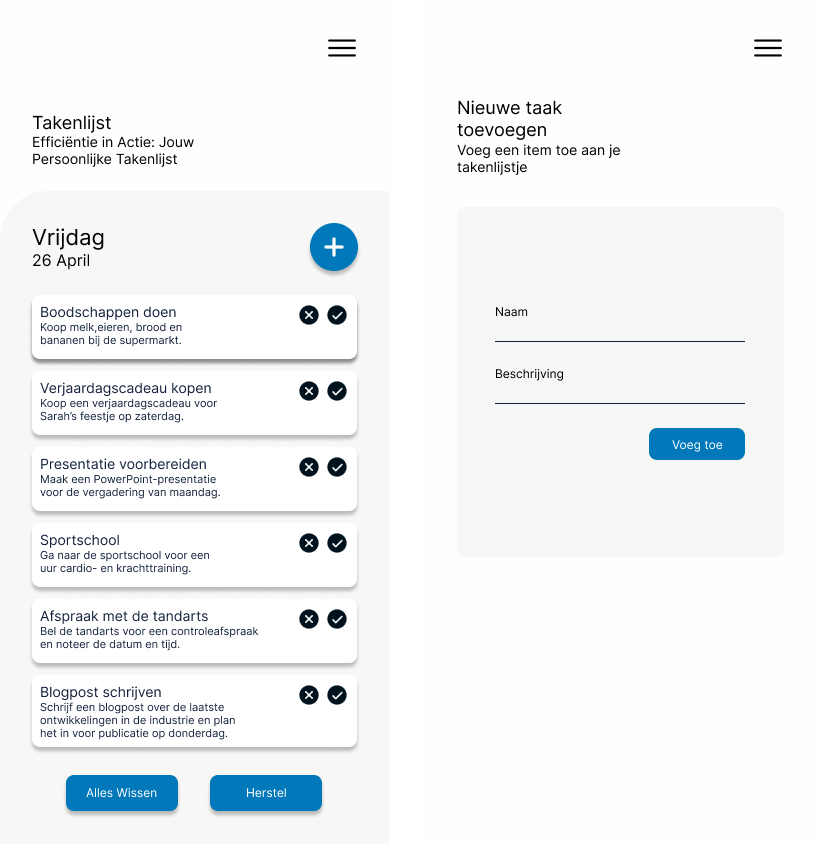
\includegraphics[scale=0.4]{todo_app_poc.png}
\\
Bron - Joeri Verhelst 
\\
\\
Daarbij zal een programmeur een andere app maken, genaamd een feedback app, die bestaat uit een formulier voor feedback dat data opslaat in AirTable.
Vervolgens zal ook via MAKE.com een e-mail gestuurd worden naar de gebruiker die feedback heeft gegeven.
Dit zorgt ervoor dat men de integratie met zowel AirTable als MAKE.com kan testen. Daarnaast zal de applicatie ook een lijst bevatten van alle feedback.
Hieronder bevindt zich ook een ontwerp van de applicatie als leidraad.
\\
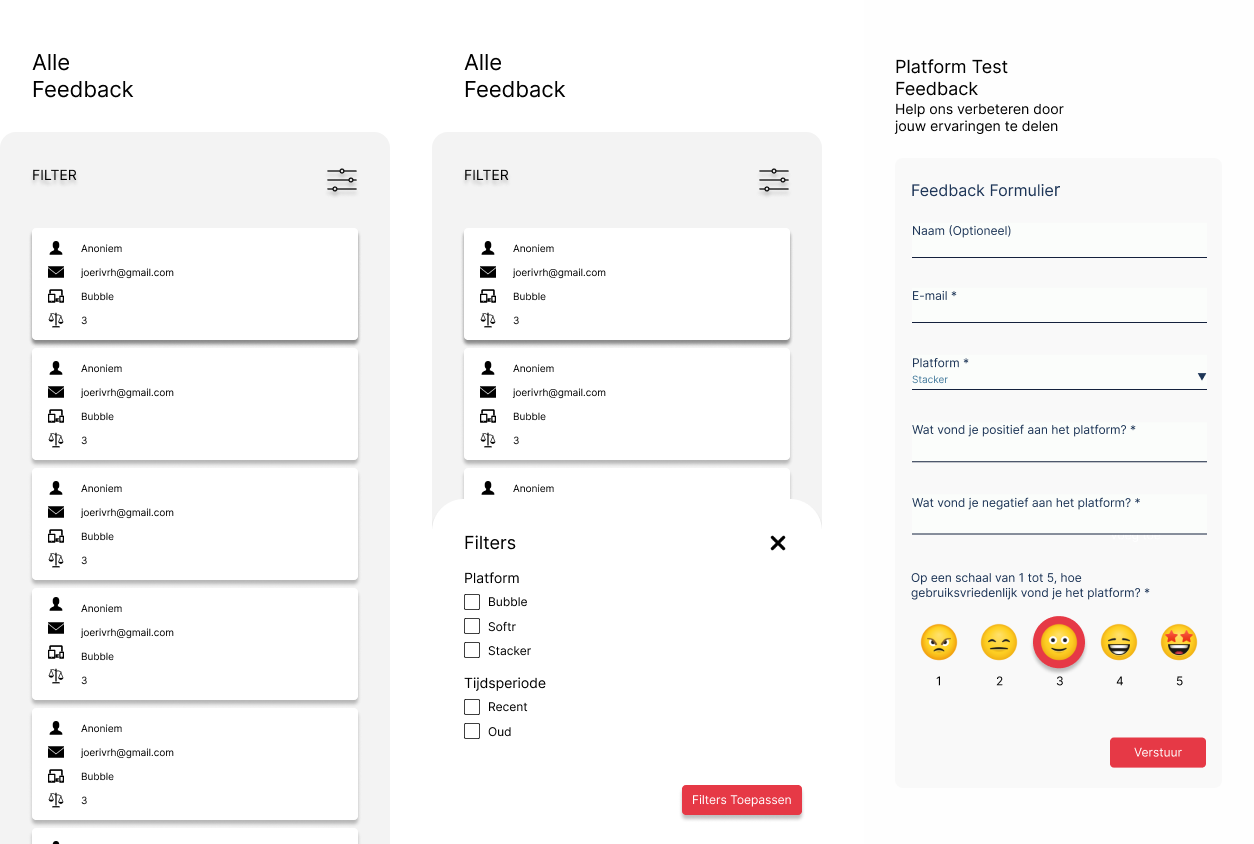
\includegraphics[scale=0.4]{feedback_app_poc.png}
\\
Bron - Joeri Verhelst 
\\
\\
Het is \textbf{belangrijk} om te vermelden dat, door de kleine steekproef, de uitgevoerde Proof of Concept niet voldoende is om een 
definitieve beslissing te nemen over welk platform het beste is voor Quivvy Solutions.

\subsection*{Benodigdheden}
Omdat alle platformen cloud-based zijn, is er een laptop en een internetverbinding nodig om de Proof of Concept uit te voeren. Vervolgens heb je ook 
een account nodig op de drie platformen; Softr, Stacker en Bubble. Deze drie platformen bieden dan ook een gratis versie aan waardoor er geen kosten aan verbonden zijn. Vervolgens zal je ook 
nog een account nodig hebben op AirTable en MAKE.com die ook een gratis versie aanbieden.

\subsection*{Uitvoer van de Proof of Concept}
\subsubsection*{Programmeur}
Voor de drie platformen te laten testen door een programmeur zal natuurlijk niet alle 3 de platformen tegelijkertijd 
kunnen getest worden, daarom zal de programmeur eerst beginnen met Softr. 
Zoals eerder vermeld zal de programmeur een feedback app moeten maken.
\\
\\
\textbf{1. Softr}
\\
Hiervoor moet hij eerst een account maken op Softr en op AirTable om de app te kunnen maken. 
Daarna kom je terecht op een overzichtelijke dashboard waar je de keuze hebt om templates te kiezen maar 
ook je eigen app te maken van nul of met AI. Bij het ontwikkelen van de app ervaarden de programmeur één probleem. 
Dit probleem was een error dat hij kreeg bij het snel verwijderen van componenten waardoor de pagina zich herstartte. 
Vervolgens merkte hij op dat de app kan hersteld worden aan de hand van de App History waarbij je terug kunt gaan 
naar een bepaalde snapshot. De programmeur heeft dan uiteindelijk de feedback app 
kunnen maken in exact 41 minuten en 54 seconden, de besteden tijd in AirTable is niet inbegrepen. 
Dit was zonder het gebruik van de AI, die Softr aanbiedt om je pagina’s voor u te maken. Vervolgens vond 
de programmeur de aantal integraties dat hij zag redelijk gelimiteerd maar de integratie met Airtable was 
zeer goed en simpel. Je kon wel helaas geen twee tabellen van de database connecteren op 1 formulier. 
Ook zag het er zeer eenvoudig uit om MAKE.com te gebruiken, maar doordat je in Softr geen 2 verschillende connecties 
kan leggen op één knop heeft de programmeur enkel AirTable gebruikt.
\\
\\
Hieronder zie je de AirTable database dat de programmeur heeft gemaakt en hoe het gebruikmaken van AirTable in Softr plaatsnam.
\\
\\
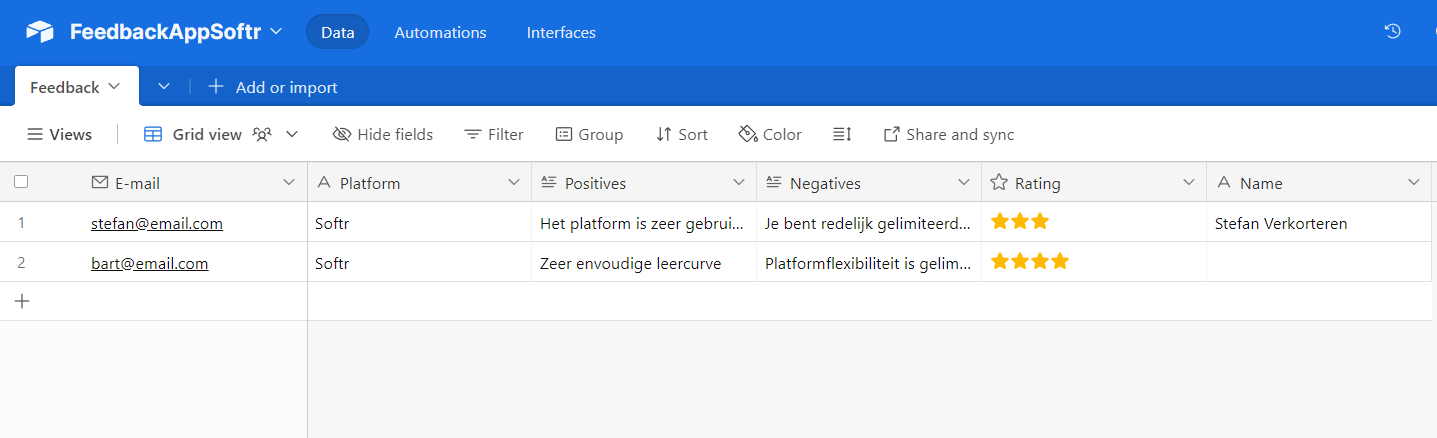
\includegraphics[scale=0.5]{softr/database-airtable-softr.png}
\\
\\
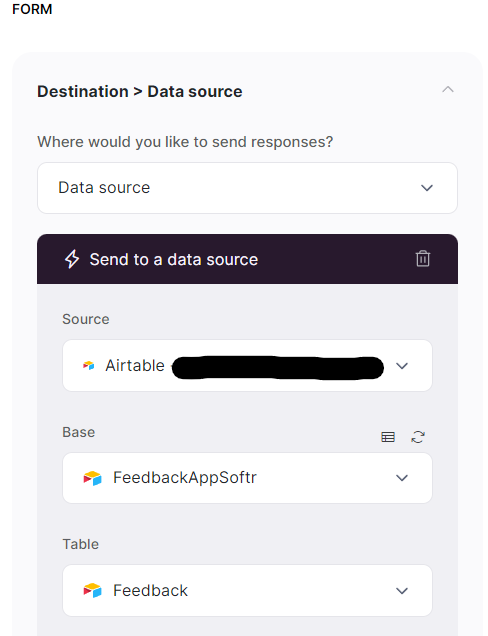
\includegraphics[scale=0.5]{softr/airtable-connectie.png}
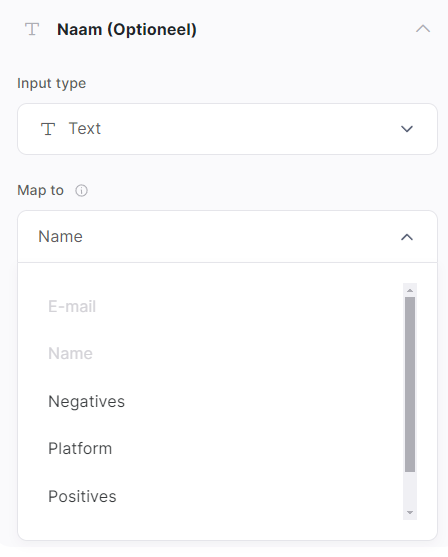
\includegraphics[scale=0.5]{softr/connectie-leggen-aan-airtable-velden.png}
\\
\\
Op vlak van platformflexibiliteit vond de programmeur het zeer matig. 
Want je kan namelijk geen meerdere acties plaatsen op een knop. 
Daarbij is het layout aanpassen van een componenten ook zeer beperkt zoals een component een border radius of shaduw geven is niet mogelijk. 
Wat de programmeur wel zeer tof vond is dat je de optie hebt om eigen custom componenten te maken via high-code en ook templates kon gebruiken.
\\
\\
Softr scoorde wel heel goed op gebruiksvriendelijkheid volgens de programmeur. 
Hij vond het zeer overzichtelijk en kon er snel mee omgaan. 
Juist was het niet mogelijk om individuele delen van een component aan te duiden om snel aan te passen. 
Alle wijzingen moeten namelijk gebeuren in het rechterpaneel waardoor je telkens moest zoeken naar het deel dat je wou aanpassen. 
Ook was je verplicht om een één template aan te duiden als startpagina bij het kiezen om een app te maken van nul, wat zeer apart was. 
\\
\\
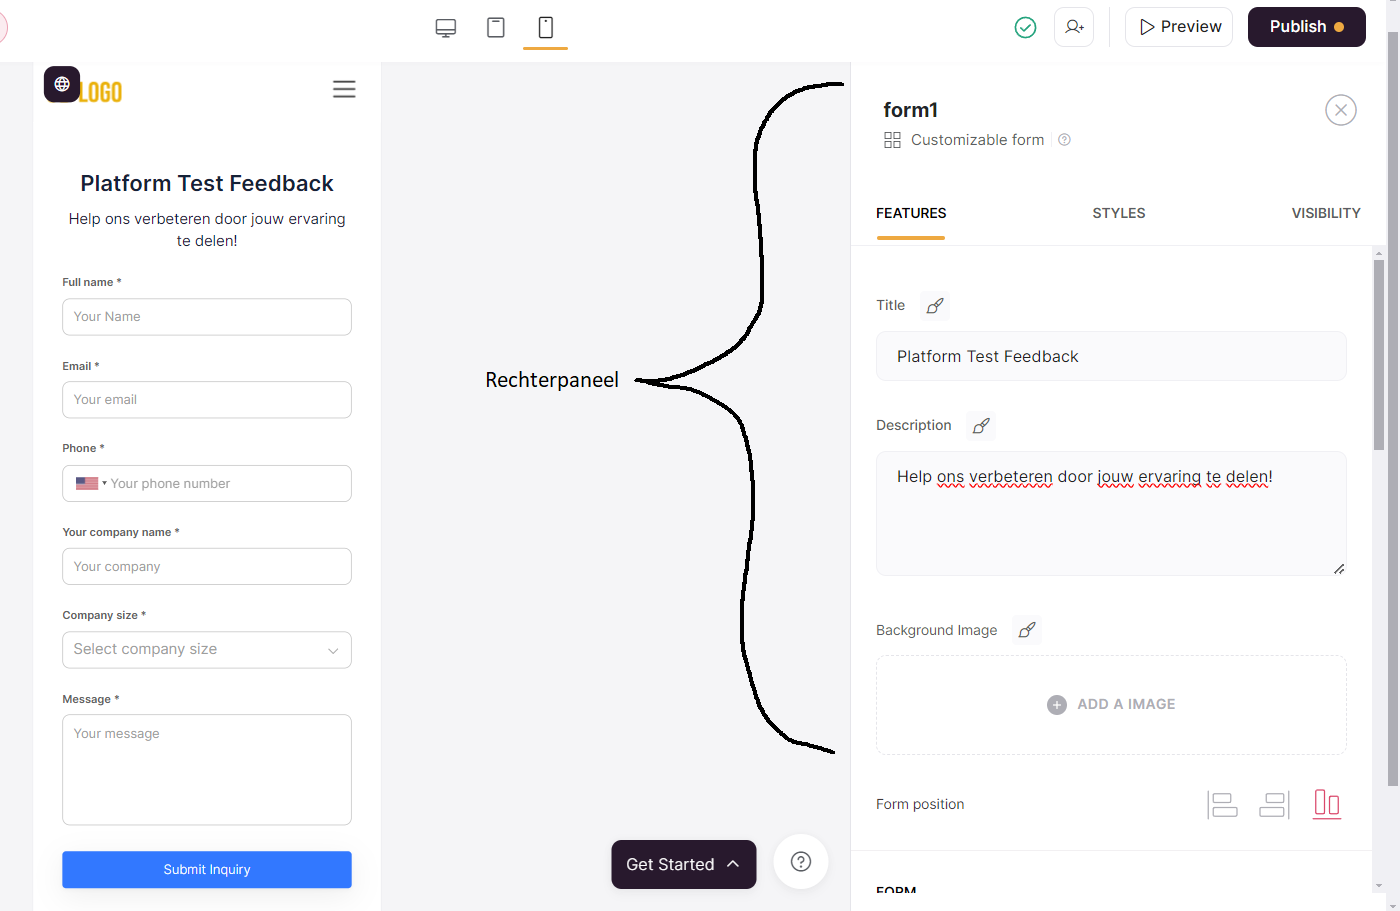
\includegraphics[scale=0.5]{softr/rechter-paneel.png}
\paragraph*{Eindresultaat}
Hieronder kunt u het eindresultaat zien van de feedback app dat gemaakt is in Softr. Door de beperkte platformflexibiliteit kon men namelijk het voorbeeld niet volledig namaken. 
Vervolgens is er ook gebruik gemaakt van een eigen component voor de titel en ondertitel. Dit component werd geschreven in HTML5 met Bootstrap.
\\
\\
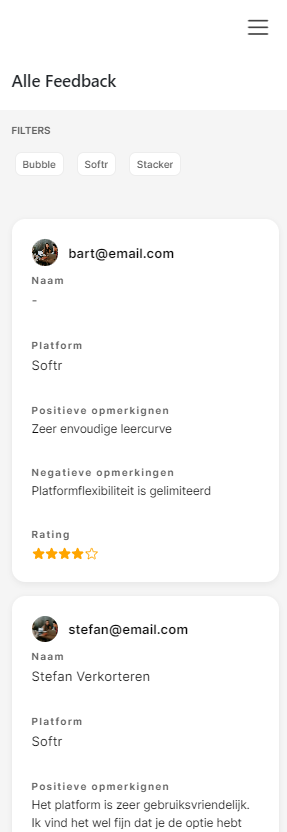
\includegraphics[scale=0.75]{softr/feedbacklijst-softr.png}
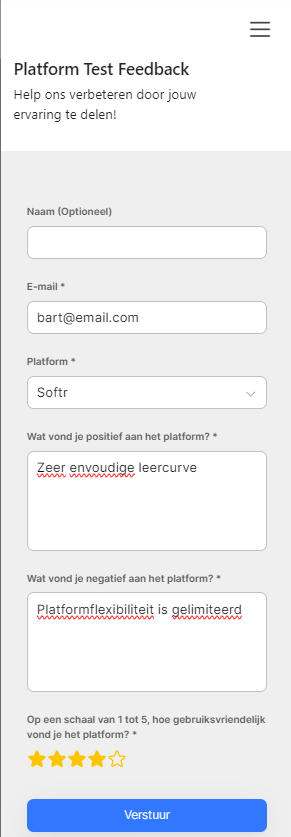
\includegraphics[scale=0.75]{softr/formulier-gemaakt-softr.png}
\paragraph*{Beoordeling}
De programmeur geeft deze app een score van 4 op 5 doordat je kon opmerken dat het platform wel redelijk gelimiteerd is, maar wel de mogelijkheid had om eigen componeten te maken. 
Hierdoor kon de programmeur achterhalen dat het maken complexe apps een echte uitdaging zou zijn met Softr, 
door de beperkte platformflexibiliteit.
\\
\\
\textbf{2. Bubble}
\\
Bij Bubble was het maken en starten van een app gelijkaardig aan Softr. Het platform op zich was snel en vlot om mee te werken. Maar bij het testen van een actie op een knop
kon het proces soms eventjes duren vooraleer de actie werd uitgevoerd. Vervolgens was het wel mogelijk bij bubble om op een knop meerdere acties te plaatsen waardoor men ook 
bij dit platform een mail versturen naar de gebruiker die feedback heeft gegeven. Hieronder kunt u dan ook de scenario vinden dat gemaakt is in MAKE.com.
\\
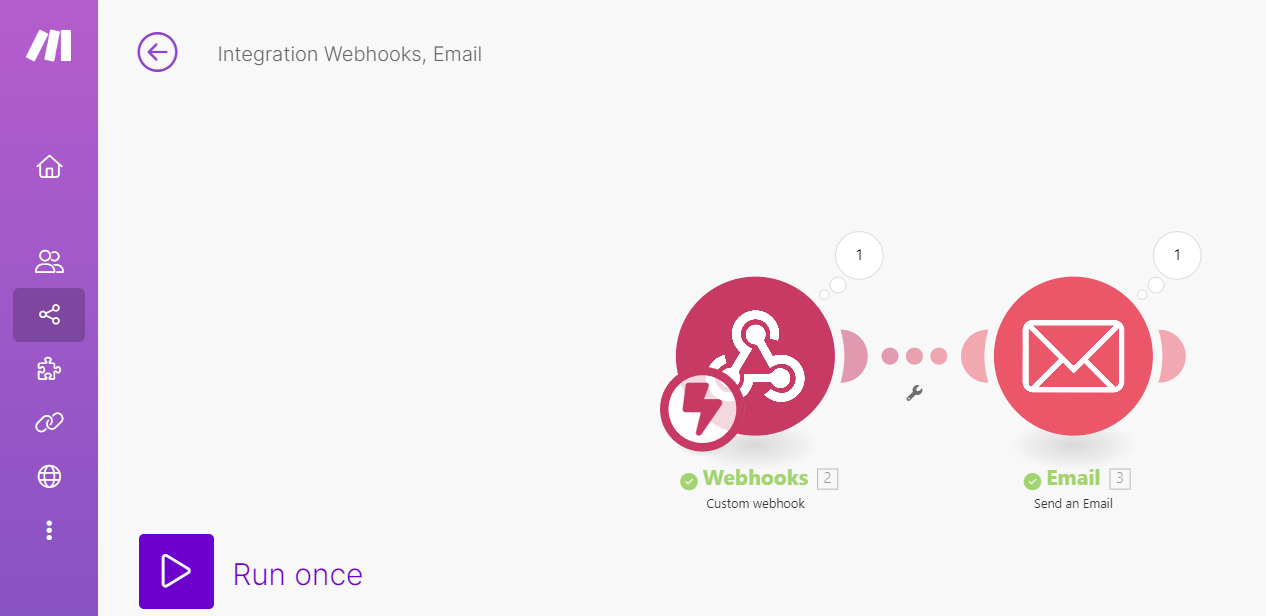
\includegraphics[scale=0.5]{bubble/make-scenario.png}
\\
\\
Het integreren met Airtable en MAKE.com was in het begin zeer verwarrend voor de programmeur. Het duurde toch wel eventjes vooraleer hij doorhad hoe hij de connectie moest leggen.
Na het zoeken naar de documentatie was het duidelijk dat je een personal acces token moet maken op Airtable om dit dan te gebruiken in Bubble. De tijd dat de programmeur nodig had 
om te integreren was 36 minuten en 3 seconden. Hieronder vind u dan ook de AirTable database dat de programmeur heeft gemaakt en de integratie met Bubble.
\\
\\
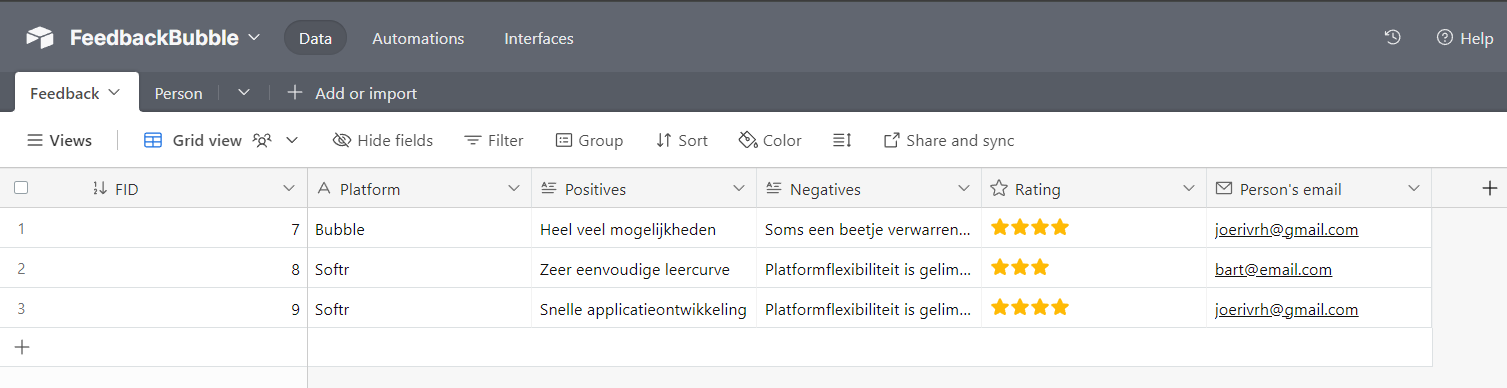
\includegraphics[scale=0.5]{bubble/AirTable-Bubble.png}
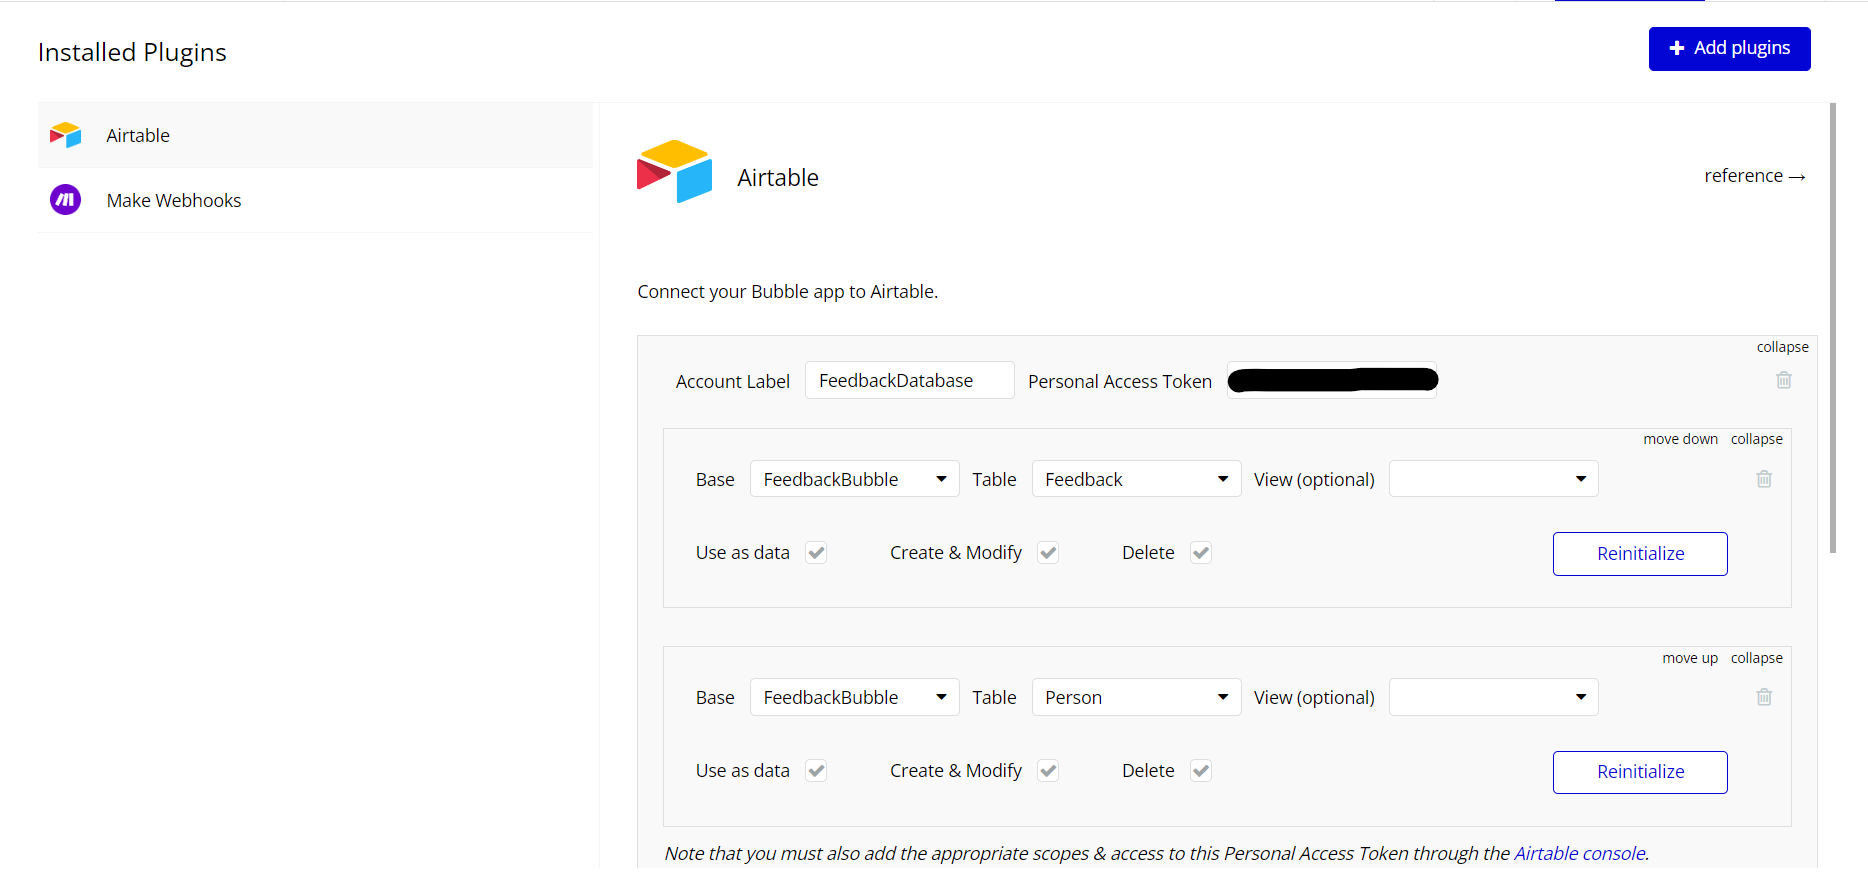
\includegraphics[scale=0.4]{bubble/integratie-airtable.png}
\\
\\
Op vlak van platformflexibiliteit was Bubble zeer goed. Je kon namelijk alles aanpassen van een component zoals de border radius, schaduw, kleur, enzovoort. 
De programmeur vond het ook duidelijk dat je met dit platform complexe apps zou kunnen maken. Daarnaast was het eerst zoeken naar hoe je acties moest plaatsen op een knop.
Je moet namelijk naar een aparte sectie gaan die alle bedrijfslogica bevat. Dit was eerst wat verwarrend voor de programmeur. De flow's of meer specifiek de acties dat je bijvoorbeeld kan doen op een 
knop was zeer flexibel, want dit zorgde ervoor dat je op een knop zowel een actie kan doen met Airtable als met MAKE.com.
\\
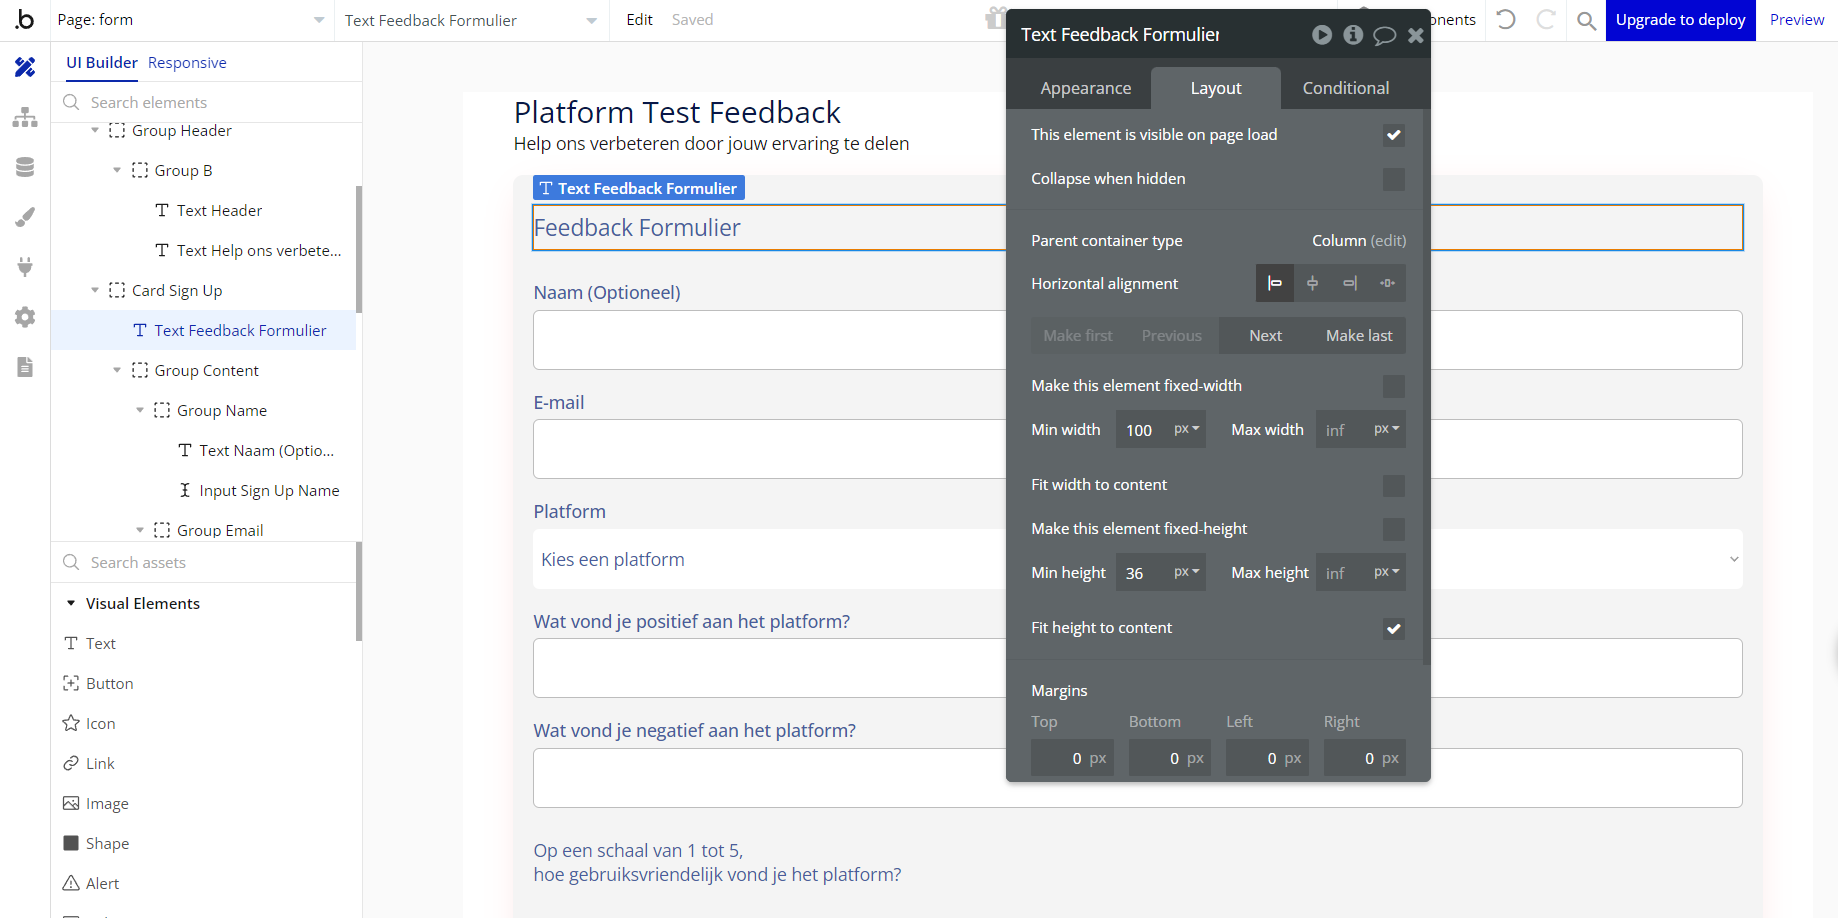
\includegraphics[scale=0.4]{bubble/element-details.png}
\\
\\
De gebruiksvriendelijkheid van de app is goed. Je komt namelijk terecht
op een scherm waarbij je kan kiezen om een app te ontwikkelen via AI of zelf van nul te beginnen. 
Vervolgens heb je de optie om direct plugins te intalleren zoals MAKE.com en Airtable. Daarna moet je de kleuren kiezen van de app.
Bij het klikken op een component krijg je direct de opties te zien die je kan aanpassen, wat zeer handig is want dit geldt voor ook delen in het component. Helaas 
kan je de live data wel niet zien in de editor maar wel bij het previewen van de app.
\\
\\
\paragraph*{Eindresultaat}
De programmeur heeft de app kunnen maken in 1 uur en 52 minutren. De oorzaak hiervan was omdat het vaak wel zoeken was hoe iets in elkaar zat, dit gelde ook bij het integreren van plugins.
Het maken van de feedbacklijst duurde het langste, namelijk 45 minuten en 18 seconden doordat het niet duidelijk was hoe je de data van Airtable moest tonen in een lijst.
Uiteindelijk is de app dat gemaakt is in Bubble zeer gelijkaardig aan het voorbeeld, door de vrijheid die Bubble beschikt. Hieronder vind u dan ook het eindresultaat van de feedback app.
\\
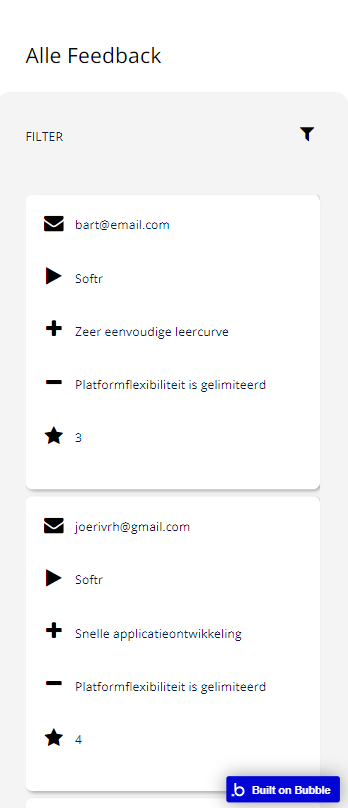
\includegraphics[scale=0.5]{bubble/feedback-lijst-bubble.png}
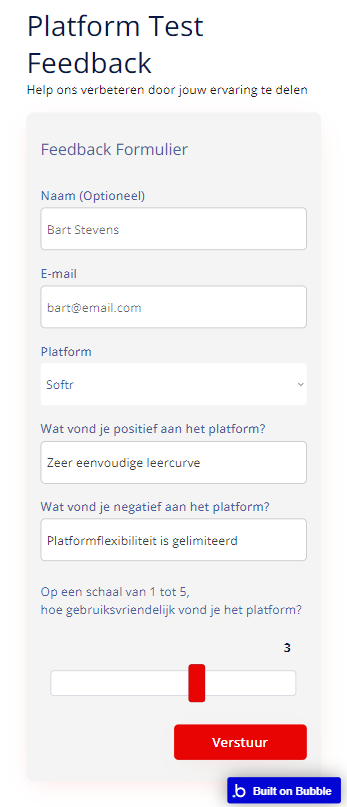
\includegraphics[scale=0.5]{bubble/formulier-resultaat-bubble.png}
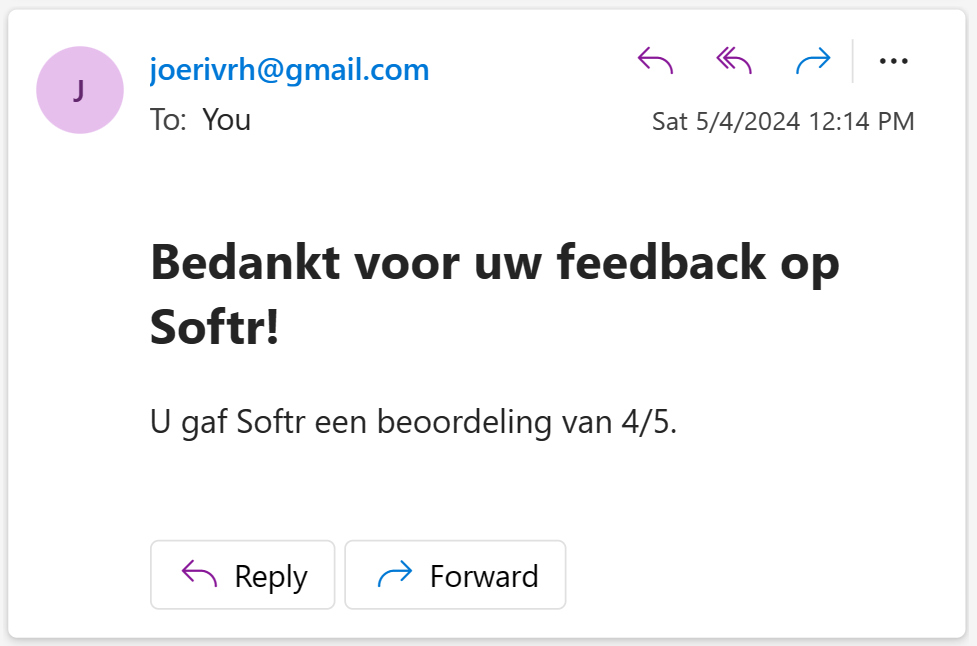
\includegraphics[scale=0.5]{bubble/ontvangen-email-bij-formulier-bubble.png}
\paragraph*{Beoordeling}
De beoordeling dat deze app heeft gekregen is 4.5 op 5. Dit komt omdat het platform zeer flexibel is. 
De beoordeling was net geen 5 op 5 omdat het soms wel zoeken was hoe je iets moest doen.
\\
\\
\textbf{3. Stacker}
\\
Bij Stacker was het proces voor het maken van een app zeer strikt en kon je niet veel aanpassen. Je moest namelijk eerst een account maken met een bedrijfsaccount.
Daarna werd er direct gevraagd om een databron te connecteren met Stacker. Hiervoor nam de programmeur AirTable waarbij het connecteren zeer snel en vlot verliep, door de duidelijke documentatie.
Helaas merkte de programmeur op, bij het ontwikkelen van de feedback app, dat het niet mogelijk was om MAKE.com te integreren met Stacker.
\\
\\
Hieronder zie je de AirTable database dat de programmeur heeft gemaakt.
\\
\\
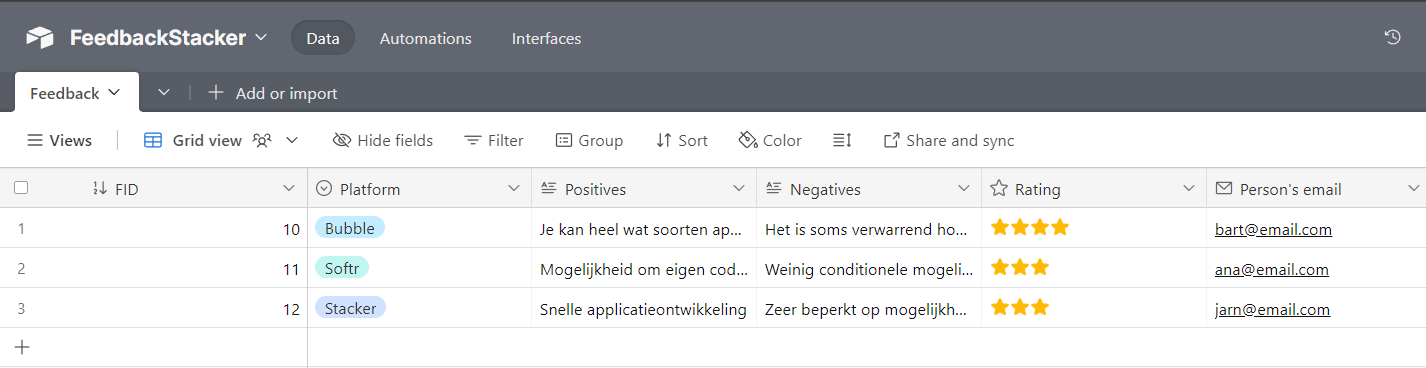
\includegraphics[scale=0.5]{stacker/airtable_stacker.png}
\\
Op vlak van platformflexibiliteit had je heel weinig vrijheid om je app aan te passen. Je kon namelijk niet de kleur kiezen van componenten want de kleuren worden gekozen
op basis van je bedrijfskleur. Daarnaast heb je ook weinig keuze in componenten. De programmeur vond dat dit platform meer bedoelt is voor het maken van CRM's en portals in plaats van 
mobiele of complexe apps.
\\
\\
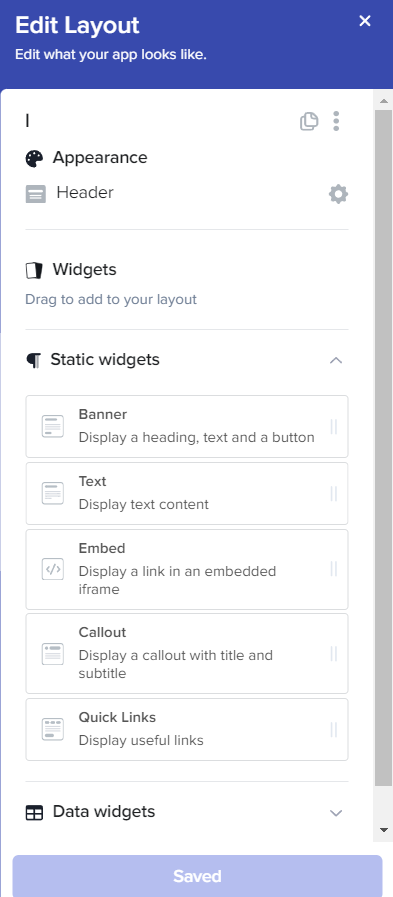
\includegraphics[scale=0.5]{stacker/componenten-stacker1.png}
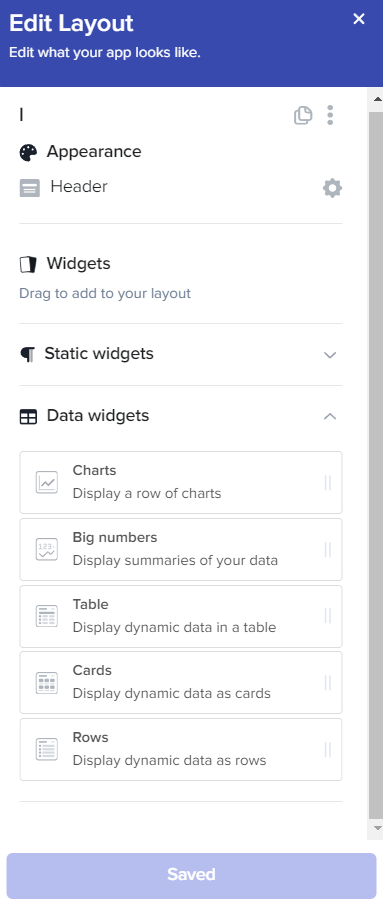
\includegraphics[scale=0.5]{stacker/componenten-stacker2.png}
\\
De programmeur vond Stacker gebruiksvriendelijk op bepaalde vlakken. Zo was het connecteren met AirTable zeer eenvoudig en duidelijk.
Ook was het leren van het platform eenvoudig door de duidelijke user interface. Maar in eerste instantie was het wel wat verwarrend om te weten waar je moest beginnen.
Het was namelijk zo dat hij niet wist of dat hij al op het scherm zat voor een app te maken of niet omdat je automatisch al een navigatiebalk hebt.
\\
\\
\paragraph*{Eindresultaat}
Door de zeer beperkte platformflexibiliteit was het namaken van het voorbeeld een grote uitdaging. Hierdoor is het namaken niet gelukt maar hij heeft wel een formulier en homescherm
kunnen ontwikkelen. Tijdens het ontwikkelen was het platform redelijk snel maar de programmeur ervaarden een crash van de laptop bij het snel klikken van verschillende knoppen op het platform.
Deze crash duurde ook ongeveer 30 seconden vooraleer alles terug normaal was. Het totaal ontwikkelen van de app heeft 26 minuten en 47 seconden geduurd. Waarbij het connecteren met AirTable 4 minuten 23 seconden duurde, het ontwikkelen van het formulier 16 minuten en 46,
en het maken van het homescherm 5 minuten en 38 seconden. Hieronder vind u dan ook het eindresultaat van de feedback app.
\\
\\
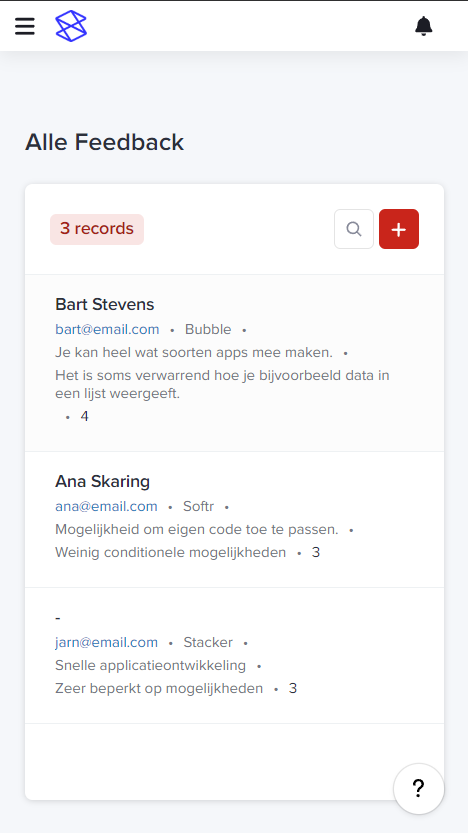
\includegraphics[scale=0.75]{stacker/feedback_lijst.png}
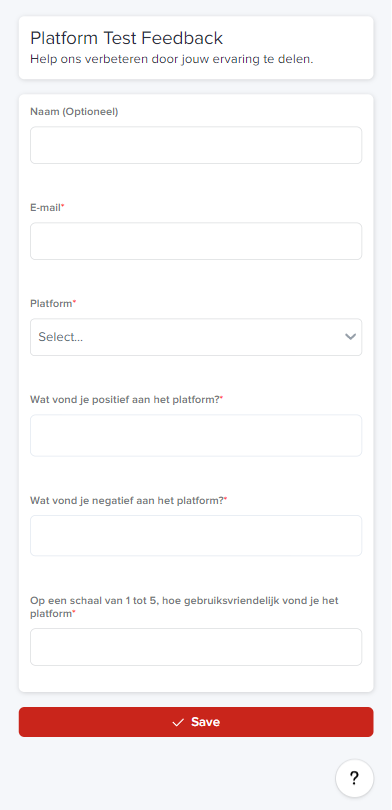
\includegraphics[scale=0.75]{stacker/formulier.png}

\paragraph*{Beoordeling}
Door de zeer matige platformflexibiliteit en de beperkte mogelijkheden van apps maken geeft de programmeur Stacker een score van 3 op 5.
De programmeur beveelden dit platform niet aan voor complexe apps te maken, maar eerder voor CRM's en portals.

\subsubsection*{Niet-programmeurs}
\subsection*{Conlusie van de Proof of Concept}

\section*{Conclusie}

